Esta seção apresenta os resultados do desenvolvimento da plataforma computacional e da aplicação do modelo de otimização EGO. A análise está organizada em três partes: (a) avaliação do desempenho do modelo substituto (\textit{Kriging}) e sua parametrização; (b) aplicação a um problema ilustrativo de dimensionamento de fundações, detalhando o fluxo de cálculo e a avaliação das restrições; e (c) descrição das funcionalidades da plataforma e da interação do usuário para obtenção de soluções otimizadas.

\subsection{Desempenho do modelo substituto}
\label{sec:desempenho_substituto}

Nesta seção, avalia-se o desempenho de um modelo substituto baseado em Regressão por Processos Gaussianos (GPR) para aproximar a função objetivo associada ao volume da fundações. A análise concentra-se em dois aspectos centrais: (\textit{i}) o impacto do fator de penalidade aplicado às restrições e (\textit{ii}) o efeito do aumento do número de amostras no conjunto de treinamento sobre a capacidade preditiva do modelo.

Diferentes funções de covariância (\textit{kernels}) foram avaliadas neste estudo, totalizando dezoito configurações distintas. Nesta seção, são apresentados os resultados referentes ao \textit{kernel} designado como \textbf{K06}, o qual consiste em uma variação parametrizada do \textit{kernel Matérn} 3/2.

Inicialmente, investigou-se a influência do fator de penalidade no comportamento da GPR. Para isso, considerou-se o \textit{kernel} \textbf{K06} e um particionamento fixo de dados ($70\%$ para treinamento e $30\%$ para teste), variando-se apenas o valor da penalidade aplicada às violações de restrição: uma penalidade suavizada ($\alpha=10^{1}$) e uma penalidade elevada ($\alpha=10^{6}$). A Figura~\ref{fig:impacto_penalidade} apresenta os gráficos de dispersão entre os valores observados e preditos para ambos os casos.

\begin{figure}[htpb!]
    \centering
    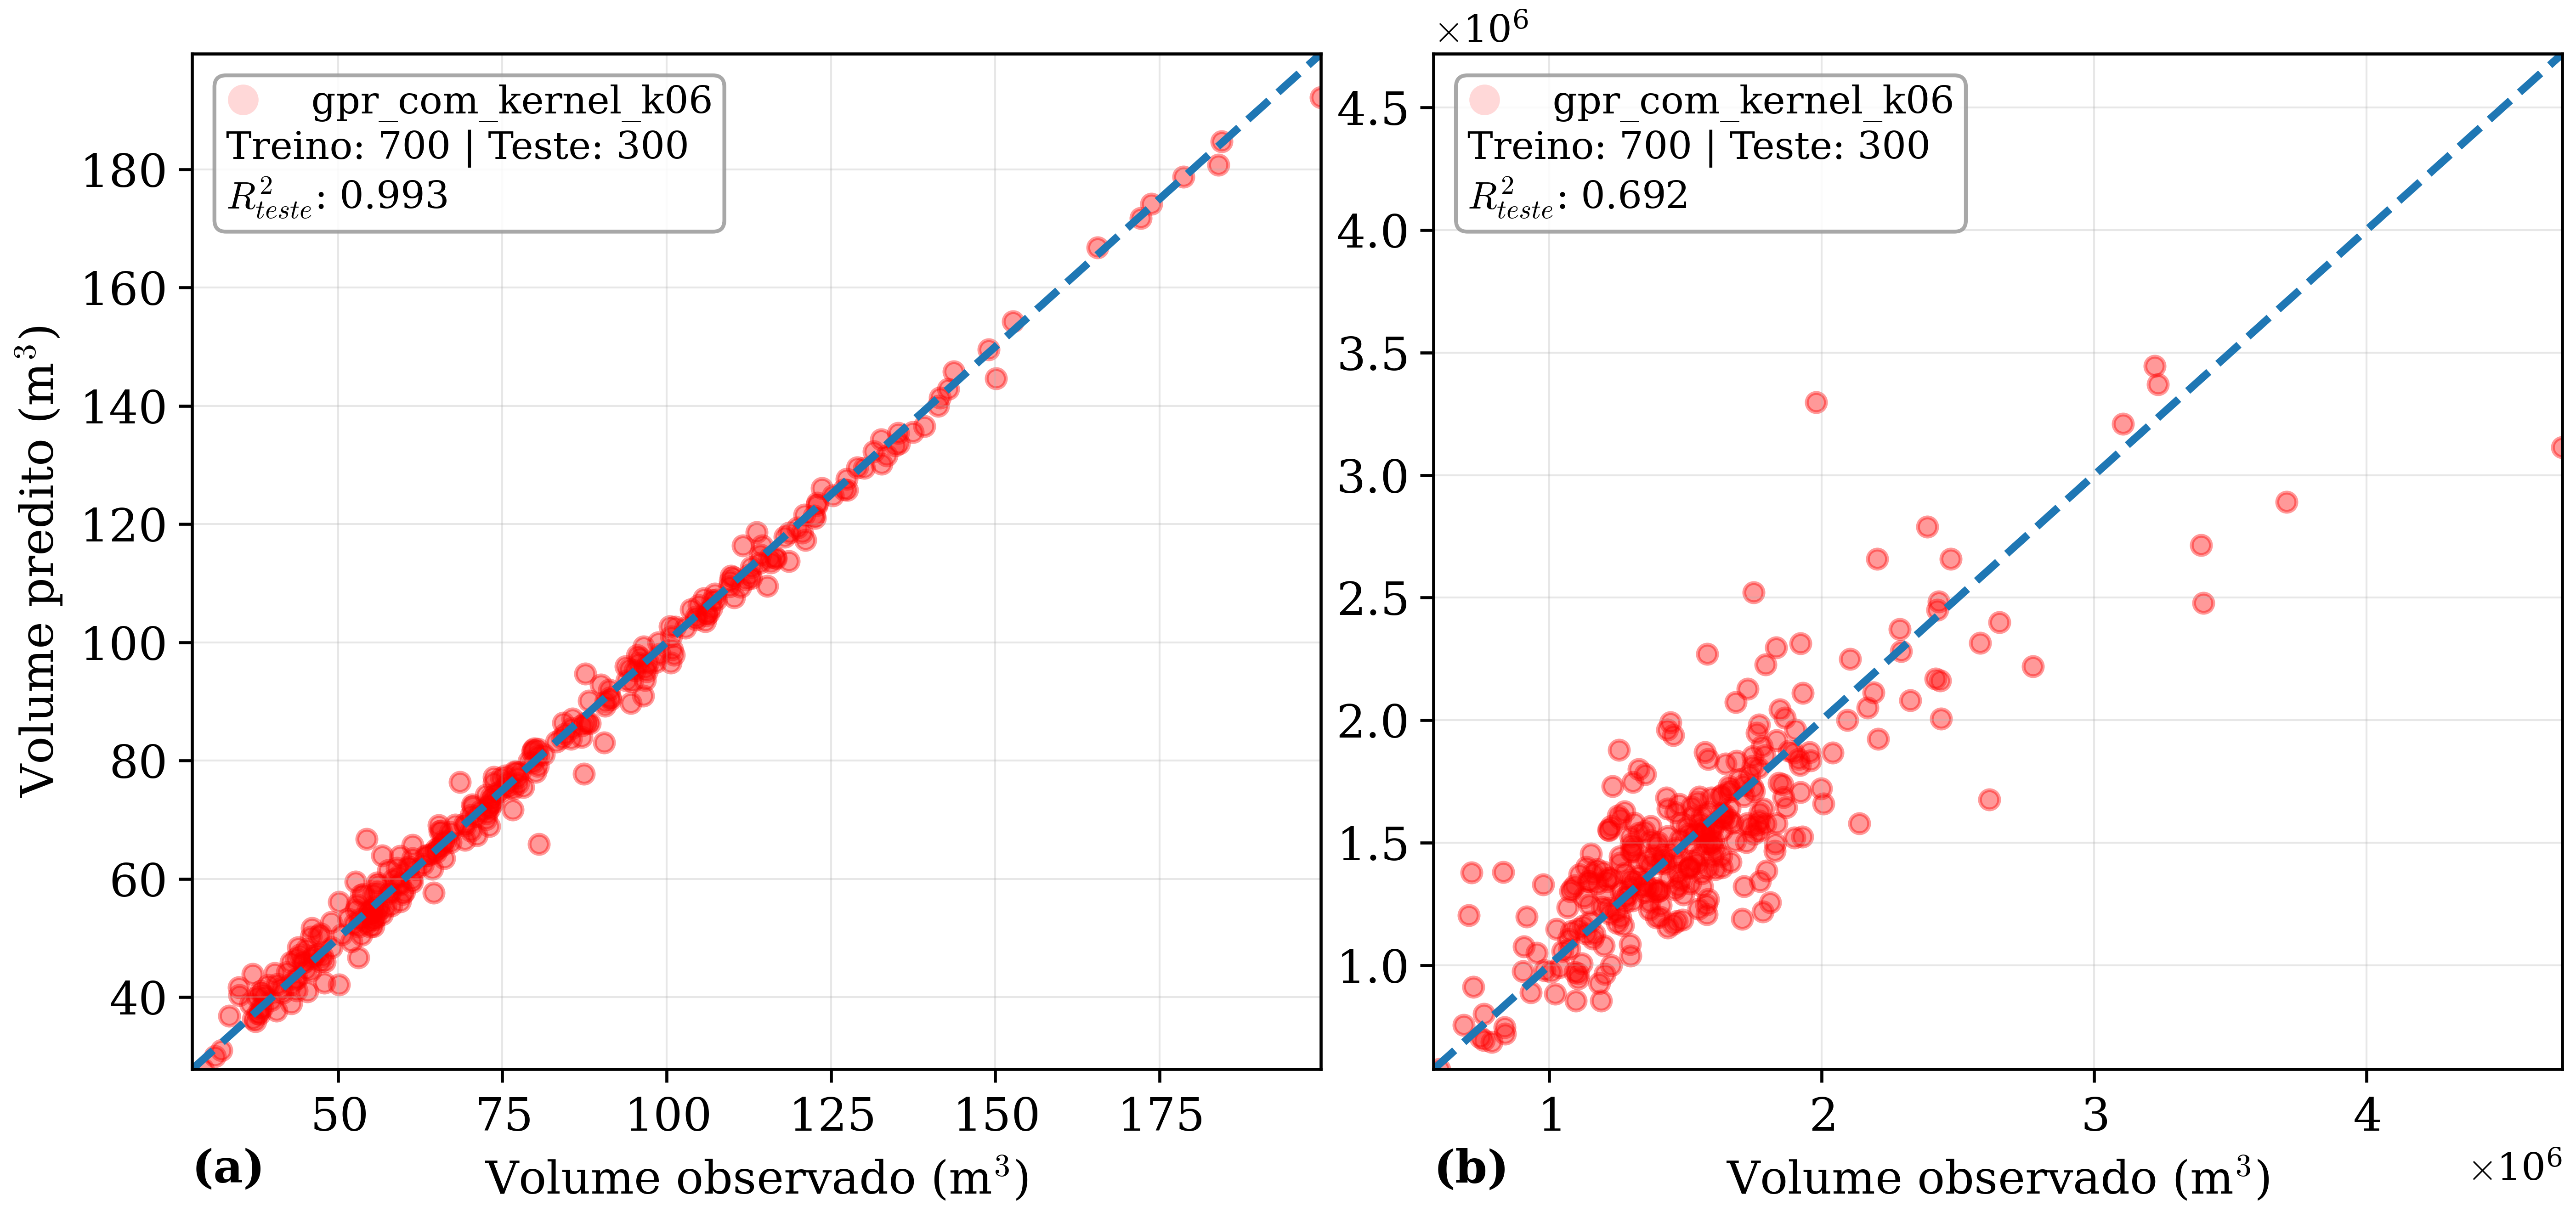
\includegraphics[width=\textwidth]{z_GPR_gpr_com_kernel_k06_pen_1e1_vs_1e6.png}
    \captionsetup{justification=centering}
    \caption{Gráficos de dispersão entre volumes observados e preditos pelo modelo GPR para o kernel k06, considerando (a) penalidade suavizada ($\alpha=10^{1}$) e (b) penalidade elevada ($\alpha=10^{6}$).}
    \label{fig:impacto_penalidade}
\end{figure}

Os resultados evidenciam que a adoção de penalidades elevadas induz uma mudança significativa na escala da função objetivo, com volumes penalizados atingindo ordens de grandeza da ordem de $10^{6}\,\mathrm{m}^3$. Essa amplificação compromete a capacidade do GPR de capturar a estrutura subjacente do problema, resultando em uma queda substancial no desempenho preditivo, com $R^2_{\mathrm{teste}} \approx 0{,}69$. Em contraste, a penalidade suavizada permite ao modelo representar adequadamente a relação entre as variáveis de decisão e o volume penalizado, alcançando valores elevados de coeficiente de determinação ($R^2_{\mathrm{teste}} \approx 0{,}99$). Esses resultados indicam que o fator de penalidade constitui um hiperparâmetro de grande importância em problemas de aprendizado ativo baseados em modelos substitutos.

Na sequência, foi avaliado o impacto do aumento do conjunto de treinamento no desempenho do GPR. Para essa análise, foram inicialmente testadas diferentes configurações de \textit{kernel} e, com base nas métricas no conjunto de teste, o \textit{kernel} \textbf{K06} foi escolhido como o mais promissor. A Figura~\ref{fig:impacto_treino} ilustra, para essa configuração (representativa do melhor desempenho), os gráficos de dispersão obtidos sob penalidade suavizada ($\alpha=10^{1}$) em dois cenários de particionamento: $90\%/10\%$ e $60\%/40\%$ (treino/teste).

\begin{figure}[htpb]
    \centering
    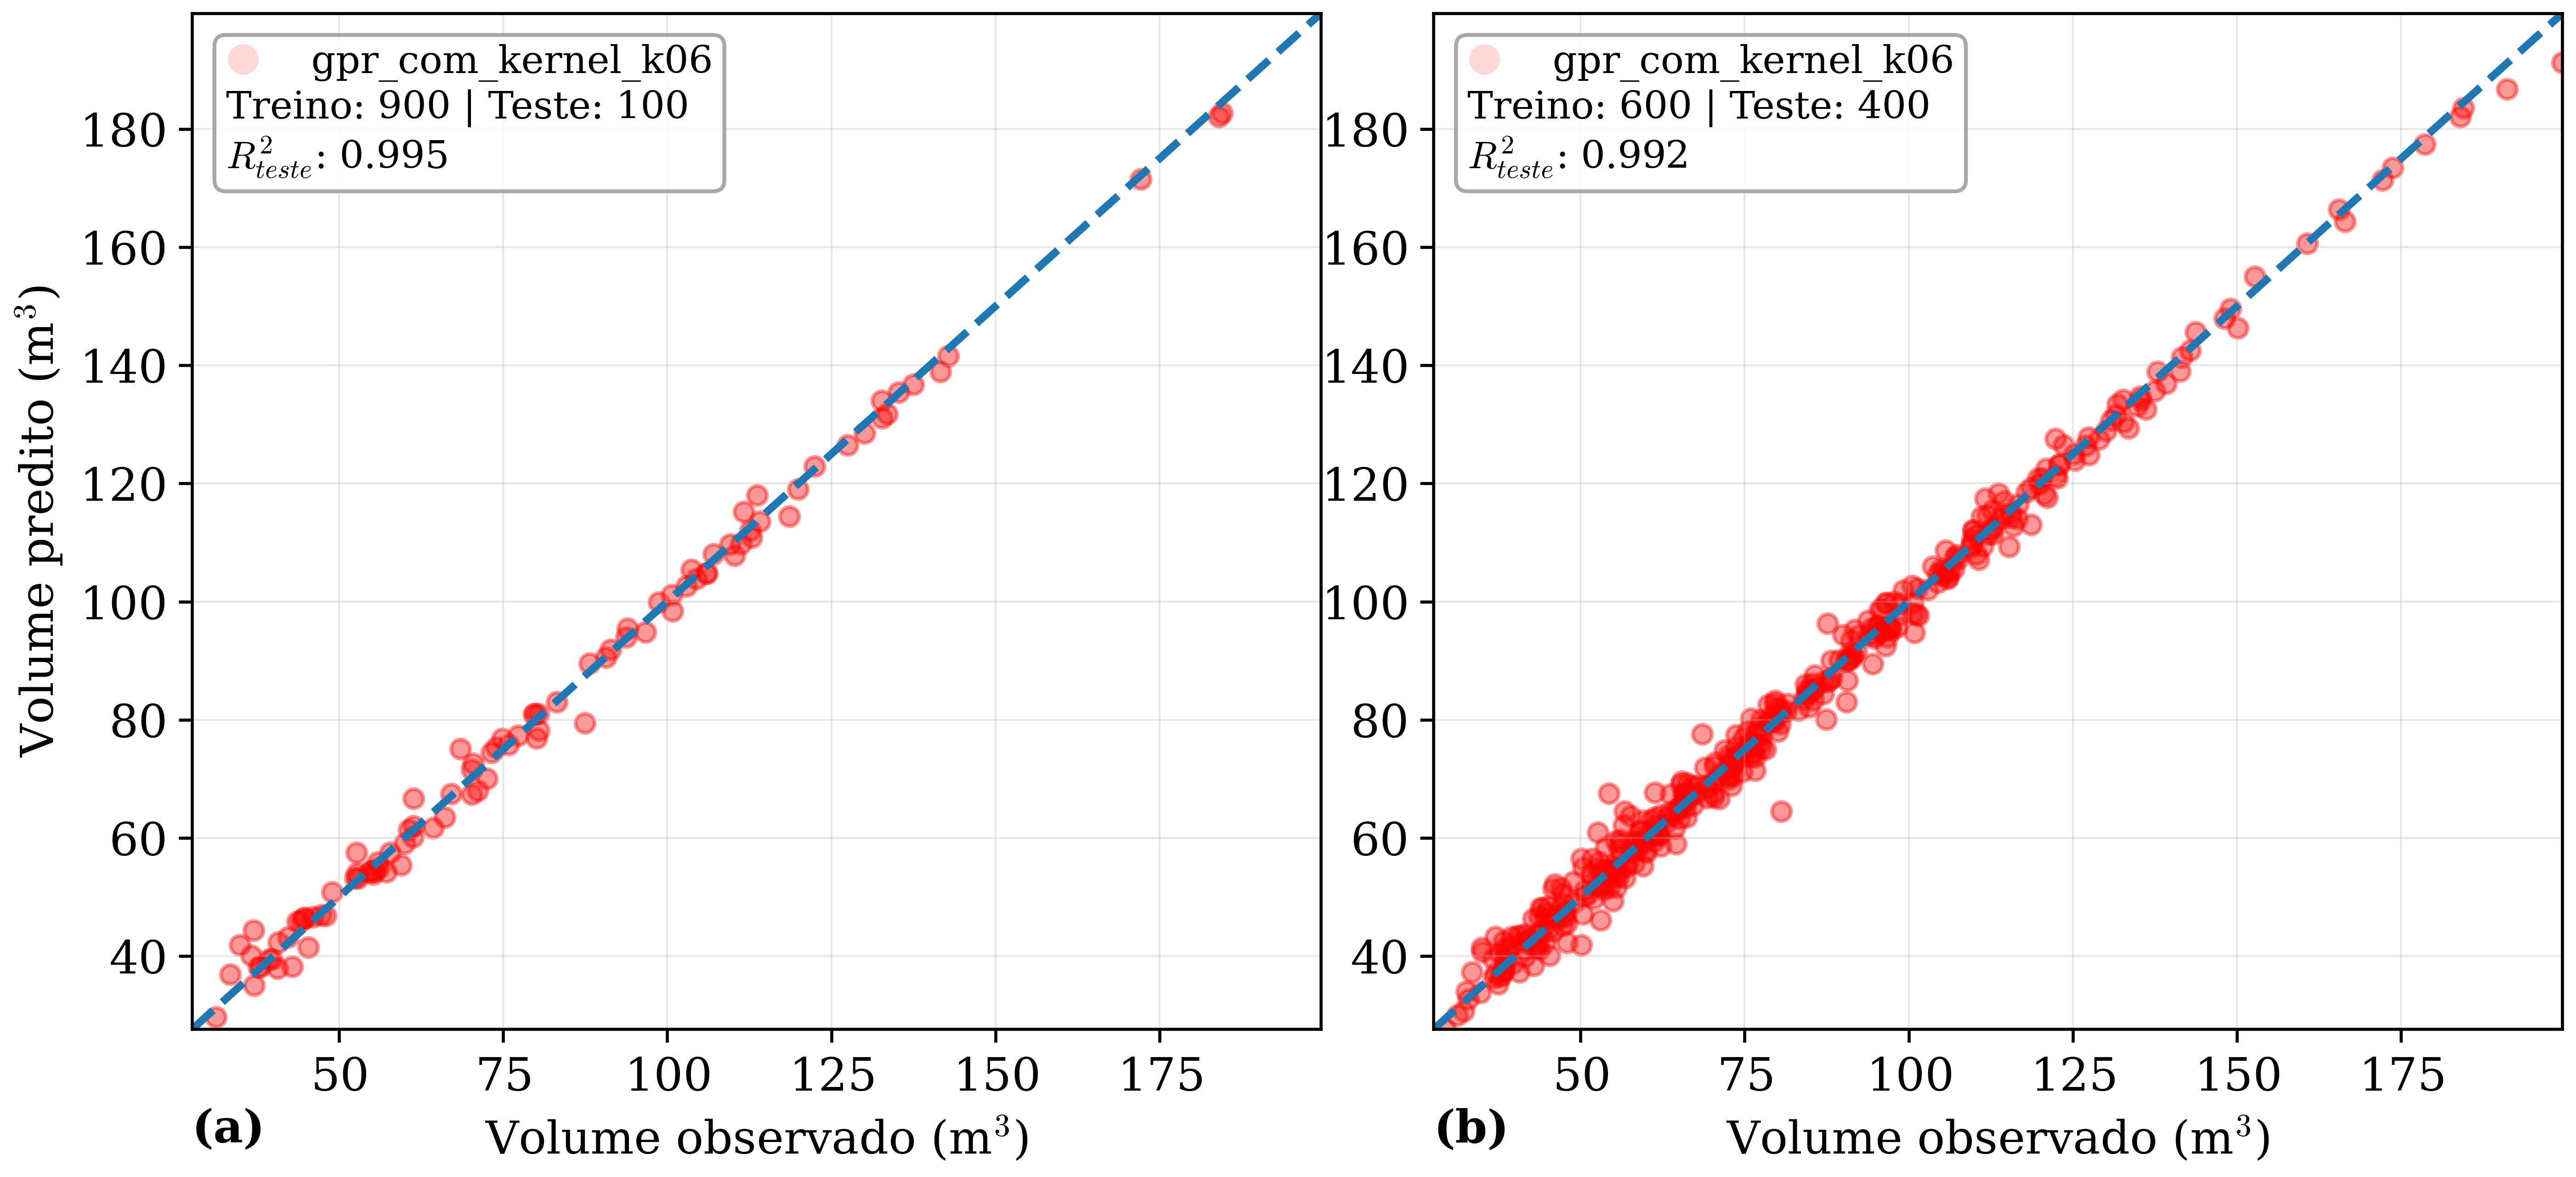
\includegraphics[width=\textwidth]{z_GPR_test_size_900_vs_600_comparison_gpr_com_kernel_k06.png}
    \captionsetup{justification=centering}
    \caption{Gráficos de dispersão entre volumes observados e preditos pelo modelo GPR para o kernel k06, considerando (a) $90\%/10\%$ (treino/teste) e (b) $60\%/40\%$ (treino/teste).}
    \label{fig:impacto_treino}
\end{figure}

Observa-se que o aumento do número de amostras de treinamento está associado a um incremento no coeficiente de determinação no conjunto de teste (de aproximadamente $0{,}992$ para $0{,}995$). Esse comportamento é consistente com o esperado em modelos estatísticos supervisionados: a ampliação do conjunto de treinamento tende a reduzir incertezas de estimação e a melhorar a aproximação da resposta, desde que as amostras sejam representativas do domínio de interesse.

Por fim, a Tabela~\ref{tab:metricas_gpr_toy_problem_all_splits} consolida as métricas de desempenho ($R^2_{\mathrm{test}}$, MAE e RMSE) para diferentes configurações de \textit{kernel}, considerando penalidade suavizada e múltiplos particionamentos treino/teste (\textit{test\_size} $\in \{0{,}10, 0{,}20, 0{,}30, 0{,}40, 0{,}50\}$). Essa análise justifica a escolha do \textit{kernel} adotado nas simulações subsequentes, destacando o desempenho superior do \textit{kernel} k06 no conjunto de teste. Ressalta-se que particionamentos com \textit{test\_size} reduzido (e.g., $0{,}10$) tendem a produzir estimativas de desempenho com maior variabilidade, uma vez que o conjunto de teste se torna menos representativo; por essa razão, a seleção do \textit{kernel} considerou a consistência das métricas ao longo dos diferentes particionamentos.

\begin{table}[H]
\centering
\caption{Métricas de desempenho dos modelos GPR para diferentes divisões treino/teste.}
\label{tab:metricas_gpr_toy_problem_all_splits}
\resizebox{\textwidth}{!}{%
\begin{tabular}{lcccccccccccccccccccc}
\toprule
\textbf{Kernel} & \textbf{Penalidade} & \textbf{Divisão} & \textbf{Treino} & \textbf{Teste} & $\mathbf{R^2_{\text{test}}}$ & \textbf{MAE}$\mathbf{_{\text{test}}}$ & \textbf{RMSE}$\mathbf{_{\text{test}}}$ \\
\midrule
gpr\_com\_kernel\_k06 & $10^{1}$ & 90/10 & 900 & 100 & 0.995 & 1.769 & 2.406 \\
gpr\_com\_kernel\_k18 & $10^{1}$ & 90/10 & 900 & 100 & 0.996 & 1.781 & 2.342 \\
gpr\_com\_kernel\_k05 & $10^{1}$ & 90/10 & 900 & 100 & 0.996 & 1.781 & 2.342 \\

\bottomrule
\end{tabular}}
\end{table}



\subsection{fluxo de cálculo para problema exemplo}\label{sec:problema_brinquedo}

Nesta Seção, descrevem-se os resultados da rotina de cálculos implementada no código, utilizados para a verificação do processo de dimensionamento e otimização aplicado a uma sapata submetida a combinações de esforços previamente definidas.

Os dados de entrada considerados no processo, que correspondem às dimensões geométricas dos pilares, às ações provenientes da superestrutura, bem como as características do solo, são apresentados nas Tabelas \ref{tab:valores_geometricos_reais} e \ref{tab:carga_atuante_real}.

\begin{table}[htbp!]
\centering
\caption{Características geométricas e do solo.}
\label{tab:valores_geometricos_reais}
\setlength{\tabcolsep}{5pt}
\begin{tabular}{ c c c c c c c}
\toprule
\textbf{Elemento} &
$\mathbf{a_p \, (m)}$ &
$\mathbf{b_p \, (m)}$ &
$\mathbf{spt}$ &
$\mathbf{solo}$ &
$\mathbf{x_g \, (m)}$ &
$\mathbf{y_g \, (m)}$\\
\midrule
P04 & 0,30 & 1,50 & 35 & argila & 32,10 & 20,37 \\
P05 & 0,25 & 1,20 & 45 & argila & 35,30 & 20,37 \\
P16 & 0,25 & 1,20 & 43 & argila & 27,75 & 18,065 \\
\bottomrule
\end{tabular}
\end{table}

% Colocar aqui a tabela de cargas 
\begin{table}[htpb!]
\centering
\caption{Cargas atuantes.}
\label{tab:carga_atuante_real}
\setlength{\tabcolsep}{5pt}
\begin{tabular}{ c c c c c c c c c c}
\toprule
\textbf{Elemento} &
$\mathbf{F_{z,c1}}$ &
$\mathbf{M_{x,c1}}$ &
$\mathbf{M_{y,c1}}$ &
$\mathbf{F_{z,c2}}$ &
$\mathbf{M_{x,c2}}$ &
$\mathbf{M_{y,c2}}$ &
$\mathbf{F_{z,c3}}$ &
$\mathbf{M_{x,c3}}$ &
$\mathbf{M_{y,c3}}$ \\
\midrule
P04 & 855,5 & -3,7 & 9,2 & 891,9 & -60,0 & 0,6 & 908,5 & -36,9 & 0,4 \\
P05 & 478,6 & -3,1 & 5,0 & 496,0 & -27,6 & 0,7 & 508,0 & -27,6 & 0,7 \\
P16 & 377,3 & -1,9 & 4,4 & 259,2 & -27,8 & 0,1 & 383,8 & 27,7 & 0,2 \\
\bottomrule
\end{tabular}
\end{table}

% tabela com cargas atuantes com unidades de medida
% \begin{table}[H]
% \centering
% \caption{Cargas atuantes}
% \label{tab:carga_atuante_real}
% \setlength{\tabcolsep}{3pt}
% \begin{tabular}{cccccccccc}
% \toprule
% \textbf{El} &
% $\mathbf{F_{z}^{c1}\,(kN)}$ &
% $\mathbf{M_{x}^{c1}\,(kN\!\cdot\! m)}$ &
% $\mathbf{M_{y}^{c1}\,(kN\!\cdot\! m)}$ &
% $\mathbf{F_{z}^{c2}\,(kN)}$ &
% $\mathbf{M_{x}^{c2}\,(kN\!\cdot\! m)}$ &
% $\mathbf{M_{y}^{c2}\,(kN\!\cdot\! m)}$ &
% $\mathbf{F_{z}^{c3}\,(kN)}$ &
% $\mathbf{M_{x}^{c3}\,(kN\!\cdot\! m)}$ &
% $\mathbf{M_{y}^{c3}\,(kN\!\cdot\! m)}$ \\
% \midrule
% P04 & 855,5 & -3,7 & 9,2 & 891,9 & -60,0 & 0,6 & 908,5 & -36,9 & 0,4 \\
% P05 & 478,6 & -3,1 & 5,0 & 496,0 & -27,6 & 0,7 & 508,0 & -27,6 & 0,7 \\
% P16 & 377,3 & -1,9 & 4,4 & 259,2 & -27,8 & 0,1 & 383,8 & 27,7 & 0,2 \\
% \bottomrule
% \end{tabular}
% \end{table}

O nome e o significado físico de cada uma das variáveis apresentadas estão descritos na Tabela \ref{tab:variaveis_descricao}.  

\begin{table}[htpb!]
    \centering
    \caption{Definição das Variáveis}
    \label{tab:variaveis_descricao}
    \begin{tabular}{lp{10cm}} % 'l' ajusta ao conteúdo, 'p{10cm}' quebra o texto se for longo
        \toprule
        \textbf{Variável} & \textbf{Descrição} \\
        \midrule
         $x_g$ & Coordenada do centro de gravidade do pilar na direção $x$. \\
         $y_g$ & Coordenada do centro de gravidade do pilar na direção $y$. \\ 
         $a_p$ & Dimensão do pilar na direção $x$. \\
         $b_p$ & Dimensão do pilar na direção $y$. \\
         $F_{z,ci}$ & Carga vertical em $kPa$, atuante no pilar, associada à combinação $i$.\\
         $M_{x,ci}$ & Momento fletor característico em $kN \cdot m$, atuante no pilar, na direção de $x$, associado à combinação de carregamento $i$.\\
         $M_{y,ci}$ & Momento fletor característico em $kN \cdot m$, atuante no pilar, na direção de $y$, associado à combinação de carregamento $i$.\\
        \bottomrule
    \end{tabular}
\end{table}

Com a finalidade de garantir a verificação independente e a rastreabilidade dos resultados, uma das soluções $(h_x, h_y, h_z)$ referente ao elemento P16, obtida ao longo do processo de otimização, foi selecionada e utilizada para a validação manual da rotina de cálculo. Considerando-se, para esta validação, a combinação de carregamento $c1$.  

Os elementos P04 e P05 terão seus resultados apresentados, porém, com a explicitação dos cálculos apenas para a verificação de sobreposição. Os valores de $h_x$, $h_y$ e $h_z$, referentes aos elementos P16, P04 e P05, bem como os parâmetros necessárias para a produção do exemplo, encontram-se na Tabela \ref{tab:valores_adotados}.

\begin{table}[htpb!]
\centering
\caption{Valores adotados para o exemplo}
\label{tab:valores_adotados}
\setlength{\tabcolsep}{10pt}
\begin{tabular}{c c c c c c}
\toprule
   \textbf{Elemento} & $\mathbf{h_x \; (m)}$ & $\mathbf{h_y \; (m)}$ & $\mathbf{h_z \; (m)}$ & $\mathbf{f_{ck} \; (MPa)}$ & $\mathbf{cob \;(cm)}$  \\
\midrule
P04 & 4,0 & 3,5 & 1,0 & 25 & 4 \\
P05 & 2,7 & 1,3 & 1,0 & 25 & 4 \\
P16 & 3,0 & 3,1 & 1,0 & 25 & 4 \\
\bottomrule
\end{tabular}
\end{table}

É importante frisar que estes valores adotados de $h_x$, $h_y$ e $h_z$ representam uma solução qualquer dentro do espaço de busca, que pode ser utilizada pelo otimizador em uma das várias tentativas para alcançar o mínimo da função objetivo e, portanto, não necessariamente correspondem a melhor solução para o elemento de fundação.

Utilizando os constantes nas Tabelas \ref{tab:valores_geometricos_reais} e \ref{tab:carga_atuante_real}, bem como os valores expressos na Tabela \ref{tab:valores_adotados}, obtêm-se os resultados apresentados a seguir

\subsubsection{Tensões solo sapata}

Dado que o solo na região do pilar P16 é argila, foi empregada a Equação \eqref{eq:tensão_rd_silte} para definição da tensão resistente do solo:

\begin{equation}
\sigma_{\text{adm}} = \frac{ 43}{50} \cdot 1000 = 860,00\;kPa
\label{eq:EL16_tensão_rd_silte}
\end{equation}

O valor da tensão devido a carga vertical, $\sigma_{Fzk}$, é definido pela Equação \eqref{eq:sigma_fz}:

\begin{equation}
    \sigma_{fz} = \frac{1,05 \cdot 377,30}{3,00 \cdot 3,10} = 42,60 \; kPa
    \label{eq:EL16_sigma_fz}
\end{equation}

Com base nesse valor, a partir das Equações \eqref{eq:sigma_max} e \eqref{eq:sigma_min} são determinadas as tensões solicitantes máxima e mínima de projeto, considerando os efeitos das excentricidades associadas aos momentos causados pela superestrutura.

\begin{equation}
\sigma_{max}^{c1} = 42,60 \cdot \left( 1 + \frac{6 \cdot |-1,90|}{377,30 \cdot 3,00} + \frac{6 \cdot 4,40}{377,30 \cdot 3,10} \right) = 43,99 \; kPa
\label{eq:EL16_sigma_max}
\end{equation}

\begin{equation}
\sigma_{min}^{c1} = 42,60 \cdot \left( 1 - \frac{6 \cdot |-1,90|}{377,30 \cdot 3,00} - \frac{6 \cdot 4,40}{377,30  \cdot 3,10} \right) = 41,21 \; kPa
\label{eq:EL16_sigma_min}
\end{equation}

Como as tensões obtidas são positivas, verifica-se que não ocorre efeito de tração entre a fundação e o solo. Portanto os valores são multiplicados por 1,30 conforme descrito na Seção \ref{Cap:proj_geometrico}.

\begin{equation}
\sigma_{max}^{c1} = 43,99 \cdot 1,30 = 57,18 \; kPa
\label{eq:EL16_sigma_max_cor}
\end{equation}

\begin{equation}
\sigma_{min}^{c1} = 41,21 \cdot 1,30 = 53,57 \; kPa
\label{eq:EL16_sigma_min_cor}
\end{equation}

Dessa forma, considera-se como referência para checagem da restrição a Equação \eqref{eq:restricao_tensão_máx}, a qual será aplicada ao resultado de tensão mais crítica, correspondente, neste caso, à tensão máxima atuante:

\begin{align}
g_{\sigma_{max}}^{c1} &= \frac{57,18}{860{,}00} - 1 = -0{,}93
    \label{eq:EL16_restricao_tensao_max} \\
g_{\sigma_{min}}^{c1} &= \frac{53,57}{860{,}00} - 1 = -0{,}94
    \label{eq:EL16_restricao_tensao_min} \\
\max &\left(g_{\sigma_{max}}^{c1},\; g_{\sigma_{min}}^{c1}\right) = -0{,}93
    \label{eq:EL16_max_tensoes}
\end{align}

Caso ocorram tensões negativas, situação indesejável no projeto de sapatas, estas seriam automaticamente convertidas para um valor de restrição positivo, conforme Equação~\eqref{eq:restricao_tensão_min}.

A Tabela~\ref{tab:tensoes_s16} sintetiza os valores das tensões atuantes no solo para cada combinação de carregamento analisada, tanto para o P16 quanto para os demais elementos, enquanto a Tabela~\ref{tab:restricoes_tensoes_s16} apresenta os resultados das respectivas verificações, formuladas na forma de funções de restrição adotadas no processo de otimização.

\begin{table}[H]
\caption{Resultados das tensões  máximas e mínimas no solo.}
\label{tab:tensoes_s16}
\centering
\begin{tabular}{ccccccc}
\toprule
\textbf{Elemento} & $\mathbf{\sigma_{\max}^{c1}\,(kPa)}$ & $\mathbf{\sigma_{\min}^{c1}\,(kPa)}$ &
$\mathbf{\sigma_{\max}^{c2}\,(kPa)}$ & $\mathbf{\sigma_{\min}^{c2}\,(kPa)}$ &
$\mathbf{\sigma_{\max}^{c3}\,(kPa)}$ & $\mathbf{\sigma_{\min}^{c3}\,(kPa)}$ \\
\midrule
P04 & 85.49  & 81.33  & 95.84  & 78.08  & 94.04  & 83.12 \\
P05 & 197.78 & 174.47 & 218.00 & 167.78 & 222.66 & 172.45 \\
P16 & 57.19  & 53.57  & 46.23  & 29.85  & 64.52  & 48.14 \\
\bottomrule
\end{tabular}
\end{table}

\begin{table}[htpb!]
\caption{Resultado das restrição das tensões solo-sapata.}
\label{tab:restricoes_tensoes_s16}
\centering
\begin{tabular}{ccccccccccc}
\toprule
\textbf{Elemento} & $\mathbf{g_{\sigma,\max}^{c1}}$ & $\mathbf{g_{\sigma,\min}^{c1}}$ & $\mathbf{g_{\sigma}^{c1}}$ &
$\mathbf{g_{\sigma,\max}^{c2}}$ & $\mathbf{g_{\sigma,\min}^{c2}}$ & $\mathbf{g_{\sigma}^{c2}}$ &
$\mathbf{g_{\sigma,\max}^{c3}}$ & $\mathbf{g_{\sigma,\min}^{c3}}$ & $\mathbf{g_{\sigma}^{c3}}$ &
$\mathbf{g_{\sigma}}$ \\
\midrule
P04 & -0.88 & -0.88 & -0.88 & -0.86 & -0.89 & -0.86 & -0.87 & -0.88 & -0.87 & -0.86 \\
P05 & -0.78 & -0.81 & -0.78 & -0.76 & -0.81 & -0.76 & -0.75 & -0.81 & -0.75 & -0.75 \\
P06 & -0.93 & -0.94 & -0.93 & -0.95 & -0.97 & -0.95 & -0.92 & -0.94 & -0.92 & -0.92 \\
\bottomrule
\end{tabular}
\end{table}

\subsubsection{Punção}

É realizada a verificação para a punção no perímetro crítico $C$. Para tanto, é a determinação da altura útil definida pela Equação \eqref{eq:altura_util}

\begin{equation}
    d = 1,00 - 0,04 = 0,96 \, m,
    \label{eq:altura_util_el16}
\end{equation}

em seguida, aplicando-se a Equação \eqref{eq:Tensão_resistente_C}, obteve-se a tensão resistente à punção no perímetro crítico $C$

\begin{equation}
 \tau_{rd,2} = 0,27 \cdot 17857,14\cdot \left( 1 - \frac{25,00}{250,00} \right) = 4339,98\;kPa,
     \label{eq:EL16_Tensão_resistente_C}
\end{equation}
 
na sequencia, por meio da Equação \eqref{eq:Tensão_solicitante_C} foi calculada a tensão solicitante de punção no perímetro~$C$

\begin{equation}
 \tau_{sd,2} = \frac{1,40 \cdot 377,30}{2 \cdot (0,25 + 1,20) \cdot 0,96} = 189,73 \; kPa.
     \label{eq:EL16_Tensão_solicitante_C}
\end{equation}

Por fim, a verificação da restrição associada à punção no perímetro~$C$ foi realizada a partir da Equação~\eqref{eq:restricao_tensao_c}, resultando no seguinte valor de restrição

\begin{equation}
g_{rd,2} = \frac{189,73}{4339,98}-1 = -0,96.
    \label{eq:EL16_restricao_tensao_c}
\end{equation}

Sendo o valor negativo um indicativo de que a tensão solicitante foi inferior à tensão resistente e por isso configura-se atendimento à restrição de punção.

Na Tabela \ref{tab:punção_tensoes_s16} encontram-se os resultados relativos às tensões de punção no perímetro crítico $C$, enquanto a Tabela \ref{tab:puncao_g_s16} mostra os valores das restrições para cada combinação, bem como o valor da restrição mais desfavorável ($g_{pun,C}$).

\begin{table}[H]
\caption{Tensões de punção.}
\label{tab:punção_tensoes_s16}
\centering
\begin{tabular}{ccccccc}
\toprule
\textbf{Elemento} &
$\mathbf{\tau_{sd,2}^{c1}\,(kPa)}$ & $\mathbf{\tau_{rd,2}^{c1}\,(kPa)}$ &
$\mathbf{\tau_{sd,2}^{c2}\,(kPa)}$ & $\mathbf{\tau_{rd,2}^{c2}\,(kPa)}$ &
$\mathbf{\tau_{sd,2}^{c3}\,(kPa)}$ & $\mathbf{\tau_{rd,2}^{c3}\,(kPa)}$ \\
\midrule
P04 & 346.56 & 4339.29 & 361.30 & 4339.29 & 368.03 & 4339.29 \\
P05 & 240.68 & 4339.29 & 249.43 & 4339.29 & 255.46 & 4339.29 \\
P16 & 189.73 & 4339.29 & 130.34 & 4339.29 & 193.00 & 4339.29 \\
\bottomrule
\end{tabular}
\end{table}

\begin{table}[htpb]
\caption{Funções de restrição da verificação à punção.}
\label{tab:puncao_g_s16}
\centering
\begin{tabular}{ccccc}
\toprule
\textbf{Elemento} &
$\mathbf{g_{2}^{c1}}$ & $\mathbf{g_{2}^{c2}}$ & $\mathbf{g_{2}^{c3}}$ & $\mathbf{g_{\mathrm{pun},C}}$ \\
\midrule
P04 & -0.92 & -0.92 & -0.92 & -0.92 \\
P05 & -0.94 & -0.94 & -0.94 & -0.94 \\
P16 & -0.96 & -0.97 & -0.96 & -0.96 \\
\bottomrule
\end{tabular}
\end{table}


\subsubsection{Sobreposição}
\label{subsec:sobreposicao_s16}

Para a verificação da sobreposição entre as fundações, são considerados os três elementos apresentados na Tabela \ref{tab:valores_geometricos_reais}. Aplicando-se os dados desses elementos nas Equações \eqref{eq:coord_x1} a \eqref{eq:coord_y4}, resulta-se nas coordenadas dos vértices dos retângulos representativos das sapatas, tal como esquematizado pela Figura \ref{fig:sobreposição}. A seguir, são apresentados os cálculos para o P16:

As coordenadas do vértice 1 são dadas por:

\begin{equation}
x_{1}= 27,75 - \frac{3,0}{2} = 26,25 \; m
    \label{eq:EL16_coord_x1}
\end{equation}

\begin{equation}
y_{1}= 18,065 - \frac{3,1}{2} =16,52 \; m
    \label{eq:EL16_coord_y1}
\end{equation}

As coordenadas do vértice 2 são dadas por:

\begin{equation}
x_{2}= 27,75 + \frac{3,0}{2} = 29,25 \; m
    \label{eq:EL16_coord_x2}
\end{equation}

\begin{equation}
y_{2}= 18,065 - \frac{3,1}{2} = 16,515 \; m
    \label{eq:EL16_coord_y2}
\end{equation}

As coordenadas do vértice 3 são dadas por:

\begin{equation}
x_{3}= 27,75 + \frac{3,0}{2} = 29,25 \; m
    \label{eq:EL16_coord_x3}
\end{equation}

\begin{equation}
y_{3}= 18,065 + \frac{3,1}{2} = 19,615 \; m
    \label{eq:EL16_coord_y3}
\end{equation}
 E por fim, as coordenadas do vértice 4 são dadas por:
 
\begin{equation}
x_{4}= 27,75 - \frac{3,0}{2} = 26,25 \; m
    \label{eq:EL16_coord_x4}
\end{equation}

\begin{equation}
y_{4}= 18,065 + \frac{3,1}{2} = 19,615 \; m
    \label{eq:EL16_coord_y4}
\end{equation}

Os mesmos cálculos são repetidos para os demais elementos considerados. As coordenadas dos vértices de cada sapata são apresentados na Tabela \ref{tab:sobreposicao_s16}.

\begin{table}[H]
\caption{Coordenadas para a verificação de sobreposição.}
\label{tab:sobreposicao_s16}
\centering
\begin{tabular}{ccccccccc}
\toprule
\textbf{Elemento} &
$\mathbf{x_1\,(m)}$ & $\mathbf{y_1\,(m)}$ &
$\mathbf{x_2\,(m)}$ & $\mathbf{y_2\,(m)}$ &
$\mathbf{x_3\,(m)}$ & $\mathbf{y_3\,(m)}$ &
$\mathbf{x_4\,(m)}$ & $\mathbf{y_4\,(m)}$  \\
\midrule
P04 & 30.10 & 18.62 & 34.10 & 18.62 & 34.10 & 22.12 & 30.10 & 22.12 \\
P05 & 33.95 & 19.72 & 36.65 & 19.72 & 36.65 & 21.02 & 33.95 & 21.02  \\
P16 & 26.25 & 16.52 & 29.25 & 16.52 & 29.25 & 19.62 & 26.25 & 19.62  \\
\bottomrule
\end{tabular}
\end{table}

Com base nos valores obtidos, verificou-se a sobreposição entre os elementos P16 e P04. Para tanto, aplicam-se as Equações \eqref{eq:overlap_x} e \eqref{eq:overlap_y}, destinadas à determinação das projeções de sobreposição entre os elementos nas direções $x$ e $y$, respectivamente:

\begin{equation}
\text{overlap}_x =  29,25 - 30,10 = -0,85 \; m < 0 \therefore \text{overlap}_y = 0,00 \; m
\label{eq:EL16_overlp_x}
\end{equation}

\begin{equation}
\text{overlap}_y = 19,62 - 18,62 = 1,00 \; m
\label{eq:EL16_overlap_y}
\end{equation}

O valor negativo obtido em $overlap_x$ indica a inexistência de sobreposição nessa direção. Consequentemente, a área de sobreposição entre as sapatas analisadas é nula, conforme identificado a seguir por meio da aplicação  da Equação \eqref{eq:area_sobreposição}:

\begin{equation}
    A_{overlap} = 0,00 \cdot 1,00 = 0,00 \; m^2
    \label{eq:EL16_area_sobreposição}
\end{equation}

Desta forma, conclui-se que não há sobreposição entre os elementos P16 e P04. No entanto, em conformidade com a lógica implementada no algoritmo, procede-se ainda à verificação formal da restrição de sobreposição por meio da Equação \eqref{eq:restricao_sobreposicao}:

\begin{equation}
g_{sobreposicao} = \frac{0}{3,00 \cdot 3,10} = 0,00
    \label{eq:EL16_restricao_sobreposicao}
\end{equation}

O valor nulo obtido confirma o atendimento à restrição de não sobreposição entre os elementos considerados.

A seguir, aplicou-se a mesma rotina de verificação para o elemento P04 em relação ao P05. Assim, com base nos valores apresentados na Tabela \ref{tab:sobreposicao_s16}, utilizam-se as Equações \eqref{eq:overlap_x} e \eqref{eq:overlap_y} para encontrar a sobreposição nas direções $x$ e $y$, respectivamente:

\begin{equation}
\text{overlap}_x =  34,10 - 22,95 = 0,15 \; m
\label{eq:EL04_overlp_x}
\end{equation}

\begin{equation}
\text{overlap}_y = 21,02 - 19,72 = 1,30 \; m
\label{eq:EL04_overlap_y}
\end{equation}


Em seguida, pela utilização da Equação \eqref{eq:area_sobreposição}, obtem-se a área de sobreposição entre os elementos:

\begin{equation}
    A_{overlap} = 0,15 \cdot 1,3 = 0,195 \; m^2
    \label{eq:EL04_area_sobreposição}
\end{equation}

A verificação de sobreposição é realizada por meio da Equação \eqref{eq:restricao_sobreposicao}, normalizando a área de interseção pela área em planta do elemento P04:

\begin{equation}
g_{sobreposicao} = \frac{0,195}{4,0 \cdot 3,5} = 0,02 
    \label{eq:EL16_restricao_sobreposicao}
\end{equation}

Para a conclusão da verificação, devem ser analisadas todaa as interações entre os elementos P16, P04 e P05, considerando-se, inclusive, a verificação mútua entre cada par de elementos (por exemplo, P04–P05 e P05–P04). Contudo, tais cálculos serão omitidos neste trabalho, podendo ser interpretados na Figura \ref{fig:sobreposicao_el16}:


A Tabela \ref{tab:sobreposicao_s16_g} apresenta o resultado da verificação de sobreposição através da analise do parâmetro $A_{overlap}$, como definido na Seção \ref{sec:method}.

\begin{table}[H]
\caption{Resultados da verificação de sobreposição.}
\label{tab:sobreposicao_s16_g}
\centering
\begin{tabular}{ccc}
\toprule
\textbf{Elemento} &
$A_{\textbf{overlap}}$ &
$\mathbf{g_{\mathbf{sobreposicao}}}$ \\
\midrule
P04 - P05 & 0,195 & 0,02 \\
P04 - P16 & 0,000 & 0,00 \\
P05 - P04 & 0,195 & 0,06 \\
P05 - P16 & 0,000 & 0,00\\
P16 - P04 & 0,000 & 0,00\\
P16 - P05 & 0,000 & 0,00 \\
\bottomrule
\end{tabular}
\end{table}


A Figura \ref{fig:sobreposicao_el16} ilustra graficamente a disposição dos elementos no plano cartesiano e a região de sobreposição:


\begin{figure}[H]
    \caption{Representação em planta dos elementos de fundação.}
    \centering
    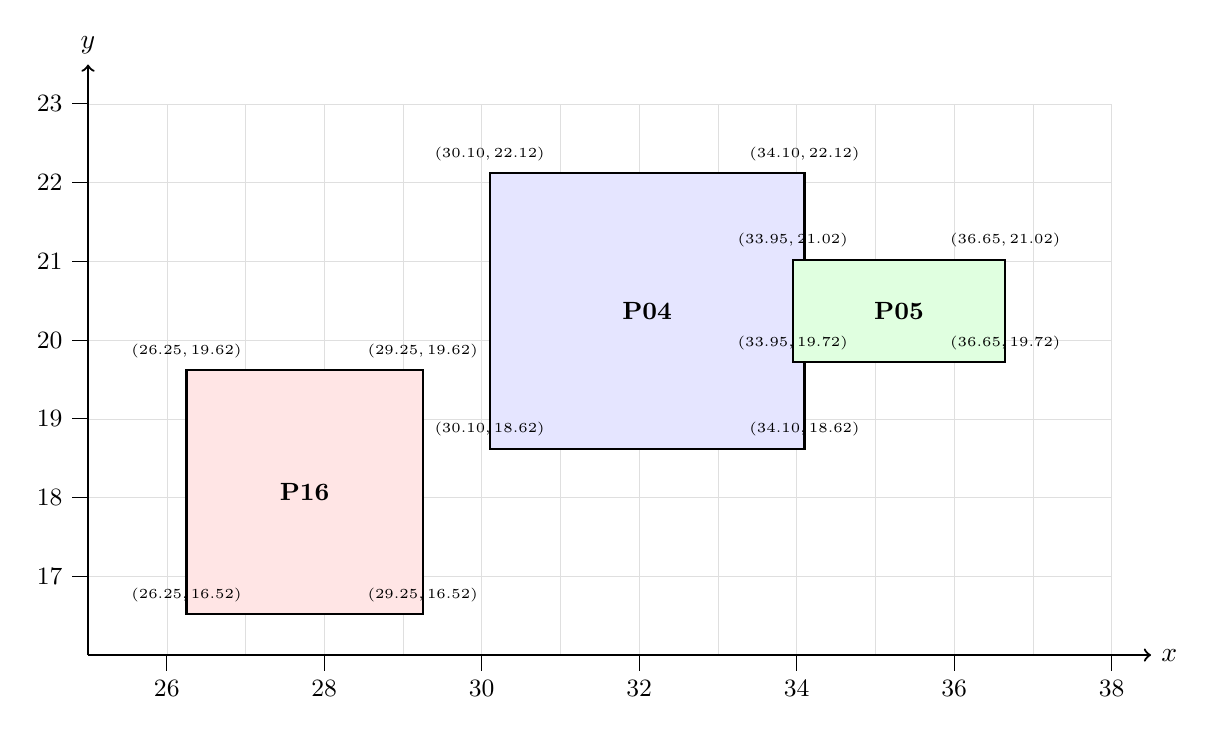
\begin{tikzpicture}[scale=1]
    
    % --------------------
    % Grade e eixos
    % --------------------
    \draw[step=1cm, gray!25, very thin] (25,16) grid (38,23);
    
    \draw[->, thick] (25,16) -- (38.5,16) node[right] {$x$};
    \draw[->, thick] (25,16) -- (25,23.5) node[above] {$y$};
    
    % Numeração dos eixos
    \foreach \x in {26,28,30,32,34,36,38}
        \draw (\x,16) -- (\x,15.8) node[below] {\small \x};
    
    \foreach \y in {17,18,19,20,21,22,23}
        \draw (25,\y) -- (24.8,\y) node[left] {\small \y};
    
    % Estilo das coordenadas
    \tikzset{
        coord/.style={font=\tiny, above=1pt, align=center}
    }
    
    % --------------------
    % Sapata 1
    % --------------------
    \draw[thick, fill=blue!10]
    (30.10,18.62) --
    (34.10,18.62) --
    (34.10,22.12) --
    (30.10,22.12) -- cycle;
    
    \node at (32.10,20.37) {\small\textbf{P04}};
    
    \node[coord] at (30.10,18.62) {(30.10,\,18.62)};
    \node[coord] at (34.10,18.62) {(34.10,\,18.62)};
    \node[coord] at (34.10,22.12) {(34.10,\,22.12)};
    \node[coord] at (30.10,22.12) {(30.10,\,22.12)};
    
    % --------------------
    % Sapata 2
    % --------------------
    \draw[thick, fill=green!12]
    (33.95,19.72) --
    (36.65,19.72) --
    (36.65,21.02) --
    (33.95,21.02) -- cycle;
    
    \node at (35.30,20.37) {\small\textbf{P05}};
    
    \node[coord] at (33.95,19.72) {(33.95,\,19.72)};
    \node[coord] at (36.65,19.72) {(36.65,\,19.72)};
    \node[coord] at (36.65,21.02) {(36.65,\,21.02)};
    \node[coord] at (33.95,21.02) {(33.95,\,21.02)};
    
    % --------------------
    % Sapata 3
    % --------------------
    \draw[thick, fill=red!10]
    (26.25,16.52) --
    (29.25,16.52) --
    (29.25,19.62) --
    (26.25,19.62) -- cycle;
    
    \node at (27.75,18.07) {\small\textbf{P16}};
    
    \node[coord] at (26.25,16.52) {(26.25,\,16.52)};
    \node[coord] at (29.25,16.52) {(29.25,\,16.52)};
    \node[coord] at (29.25,19.62) {(29.25,\,19.62)};
    \node[coord] at (26.25,19.62) {(26.25,\,19.62)};
    
    \end{tikzpicture}
    \label{fig:sobreposicao_el16}
\end{figure}




\subsubsection{Geometria}
\label{subsec:geometria_s16}

Para a verificação geométrica, aplicam-se as Equações \eqref{eq:checagem_geometria_x} e \eqref{eq:checagem_geometria_y}:

\begin{equation}
g_{geometria,x} = 1 + \frac{2 \cdot 0,05 }{0,25} -  \frac{3,00}{0,25} =  -10,6 \; <0
    \label{eq:el16_checagem_geometria_x}
\end{equation}

\begin{equation}
g_{geometria,y} = 1 + \frac{2 \cdot 0,05 }{1,20} -  \frac{3,10}{1,20}  = -1,5 \; < 0
    \label{eq:el16_checagem_geometria_y}
\end{equation}

Os valores negativos obtidos para \(g_{\text{geometria},x}\) e \(g_{\text{geometria},y}\) indicam que as restrições geométricas são plenamente satisfeitas, uma vez que as dimensões da sapata excedem de forma significativa as dimensões do pilar nas duas direções analisadas. Dessa forma, não há violação das condições geométricas impostas. Os resultados da verificação geométrica nas direções $x$ e $y$ são apresentados na Tabela \ref{tab:geometria_s16}, bem como aquele que configura o pior caso.


\begin{table}[H]
\caption{Resultados da verificação de geometria.}
\label{tab:geometria_s16}
\centering
\begin{tabular}{cccc}
\toprule
\textbf{Elemento} &
$\mathbf{g_{\mathrm{geom},x}}$ & $\mathbf{g_{\mathrm{geom},y}}$ & $\mathbf{g_{\mathrm{geom}}}$ \\
\midrule
 P04 & -12,00 & -1,27 & -1.27 \\
 P05 & -9,40  & 0,00  & 0,00  \\
 P16 & -10.60 & -1.50 & -1.50 \\
\bottomrule
\end{tabular}
\end{table}

Nota-se que, para o P05, a restrição $g_{geom,y}$ igual a zero indica que a dimensão adotada chegou ao limiar da viabilidade. Contudo, não configura um descumprimento da restrição.

\subsection{O \textit{framework }FUNDAAI}

Neste trabalho, desenvolveu-se a plataforma web \textbf{FundaAI} para dimensionamento automatizado de fundações, acessível em \url{https://fundaai.streamlit.app/}. A ferramenta implementa a metodologia proposta, proporcionando uma interface prática para aplicação em projetos reais. Ela foi implementada em um ambiente \textsc{STREAMLIT} \cite{streamlit2024}, um \textit{framework Python} de código aberto que permite criar aplicativos de dados. 

A ferramenta possibilita a importação de uma planilha de dados contendo informações da planta de fundações, incluindo dados geométricos dos elementos, características geotécnicas do solo e combinações de carregamento provenientes da superestrutura, além de parâmetros adicionais definidos diretamente pelo usuário. Esses parâmetros correspondem ao cobrimento ($cob$) à resistência característica à compressão do concreto ($f_{ck}$) em MPa e às dimensões máximas e mínimas da sapata ou do conjunto de sapatas a ser dimensionado. 

Os parâmetros citados anteriormente referem-se aos parâmetros do modelo mecânico da sapata. Além disso, o usuário define o número de iterações do algoritmo a ser empregado, bem como o tamanho da população que será empregada a cada geração para a busca da solução ótima.

O funcionamento da plataforma envolve, inicialmente, a inserção da planilha de dados e dos parâmetros de dimensionamento pelo usuário. Após essa etapa, a execução do algoritmo é iniciada, realizando assim o dimensionamento geométrico dos elementos de fundação conforme descrito na Seção \ref{sec:sapata}.

Após a conclusão da rotina de cálculos e do processo de dimensionamento, a plataforma disponibiliza duas planilhas de resultados. A primeira contém as dimensões ótimas determinadas para cada elemento analisado e a segunda apresenta o conjunto completo dos valores finais das verificações efetuadas, correspondentes à solução considerada ótima.

Com o objetivo de demonstrar a operacionalidade da ferramenta \textbf{FundaAI}, esta seção descreve a interface gráfica da plataforma, detalhando suas funcionalidades e fluxo de interação. Adicionalmente, são apresentados resultados de processos de otimização ilustrativos, baseados no problema-exemplo discutido na seção anterior, que evidenciam a eficácia da abordagem proposta.

A interface da ferramenta foi estruturada de forma intuitiva, de modo a guiar o usuário ao longo das etapas necessárias para a execução do dimensionamento. A Figura \ref{fig:pag_web_inicial} apresenta a página inicial, onde pode-se definir o idioma e ver as informações necessárias para o uso, além de baixar um exemplo de arquivo de entrada.

\begin{figure}[htpb!]
    \centering
    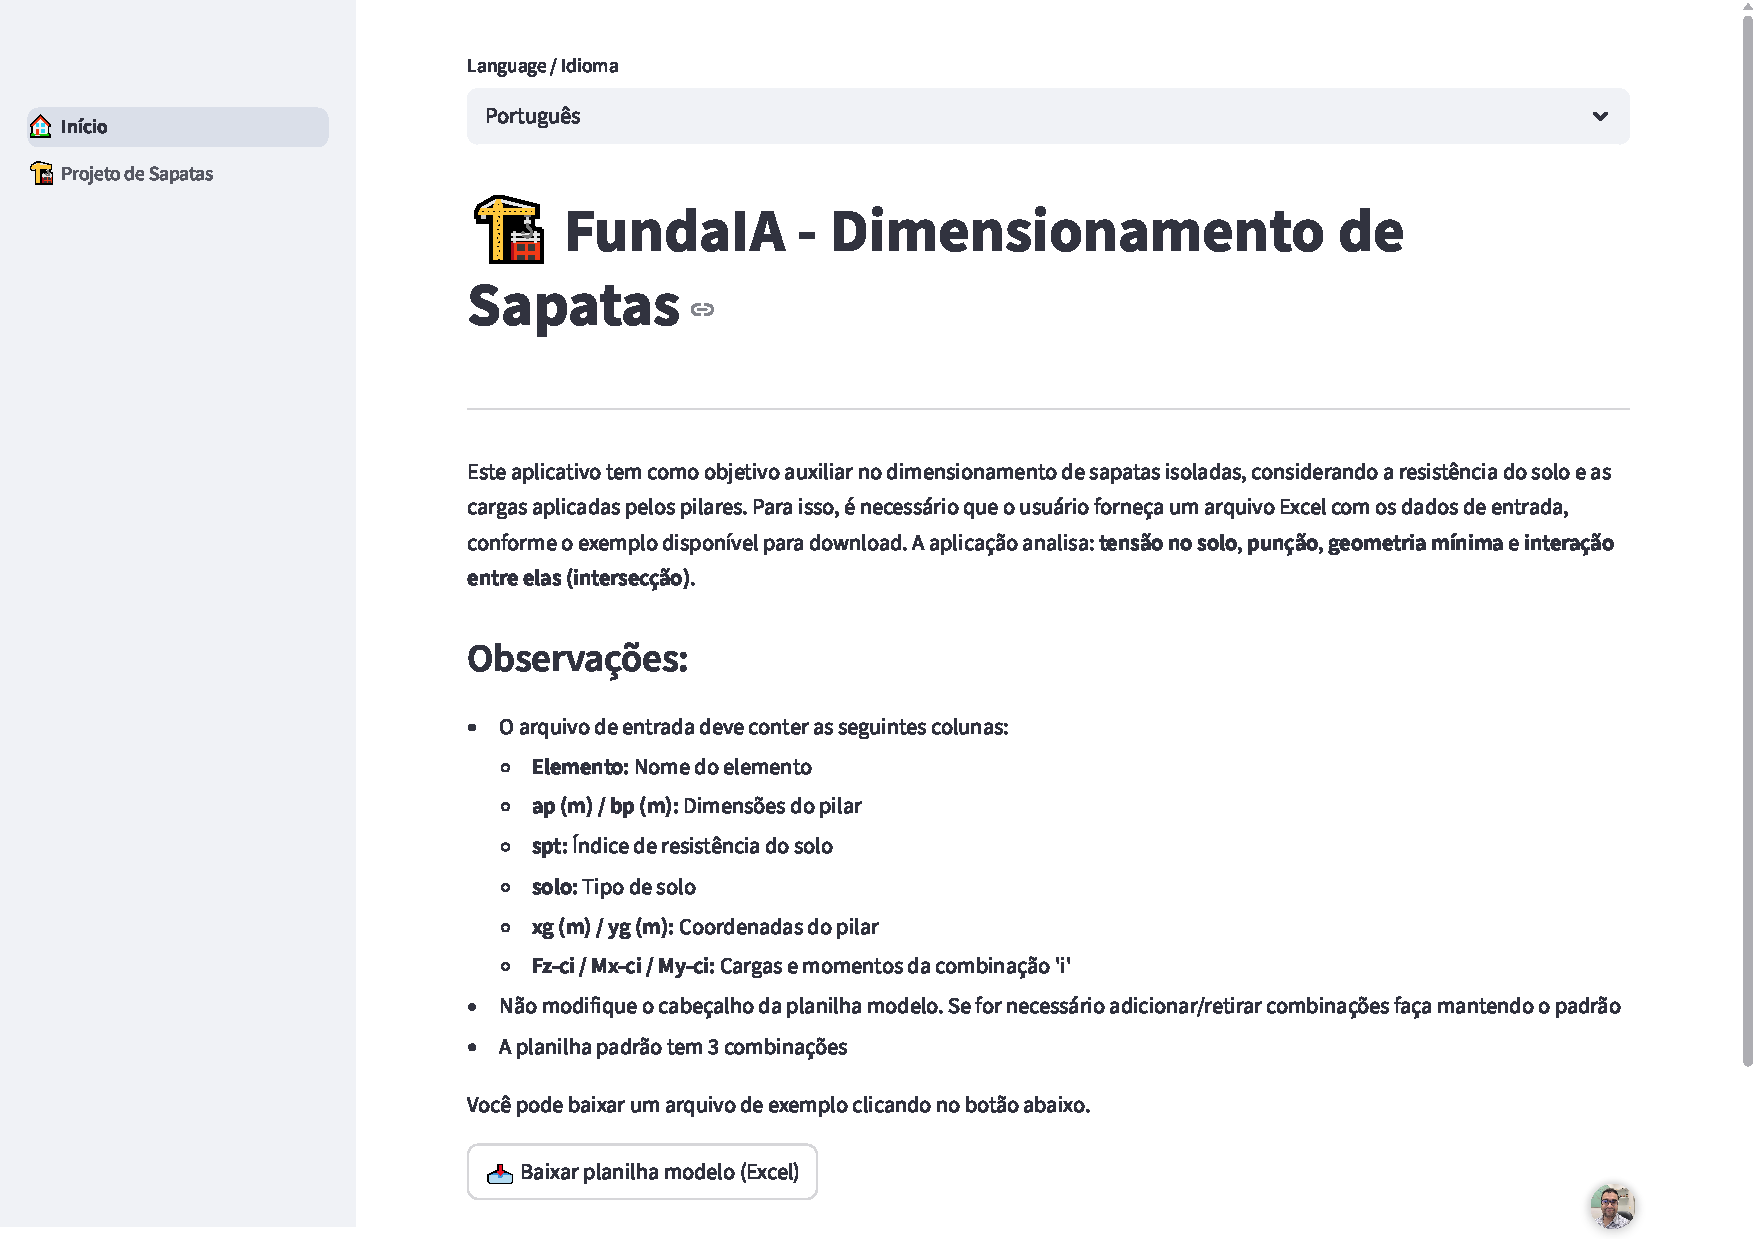
\includegraphics[width=1\linewidth]{figuras/pag_web_inicial.pdf}
    \caption{Página inicial da ferramenta \textit{web}.}
    \label{fig:pag_web_inicial}
\end{figure}

Entrando na aba "Projeto de Sapatas" (ver Figura \ref{fig:pag_web_dados}), o usuário tem acesso aos parâmetros que devem ser definidos. Na mesma aba, tem-se o local para inserção da planilha de entrada, em destaque na Figura \ref{fig:pag_web_insercao}.

\begin{figure}[htpb!]
    \centering
    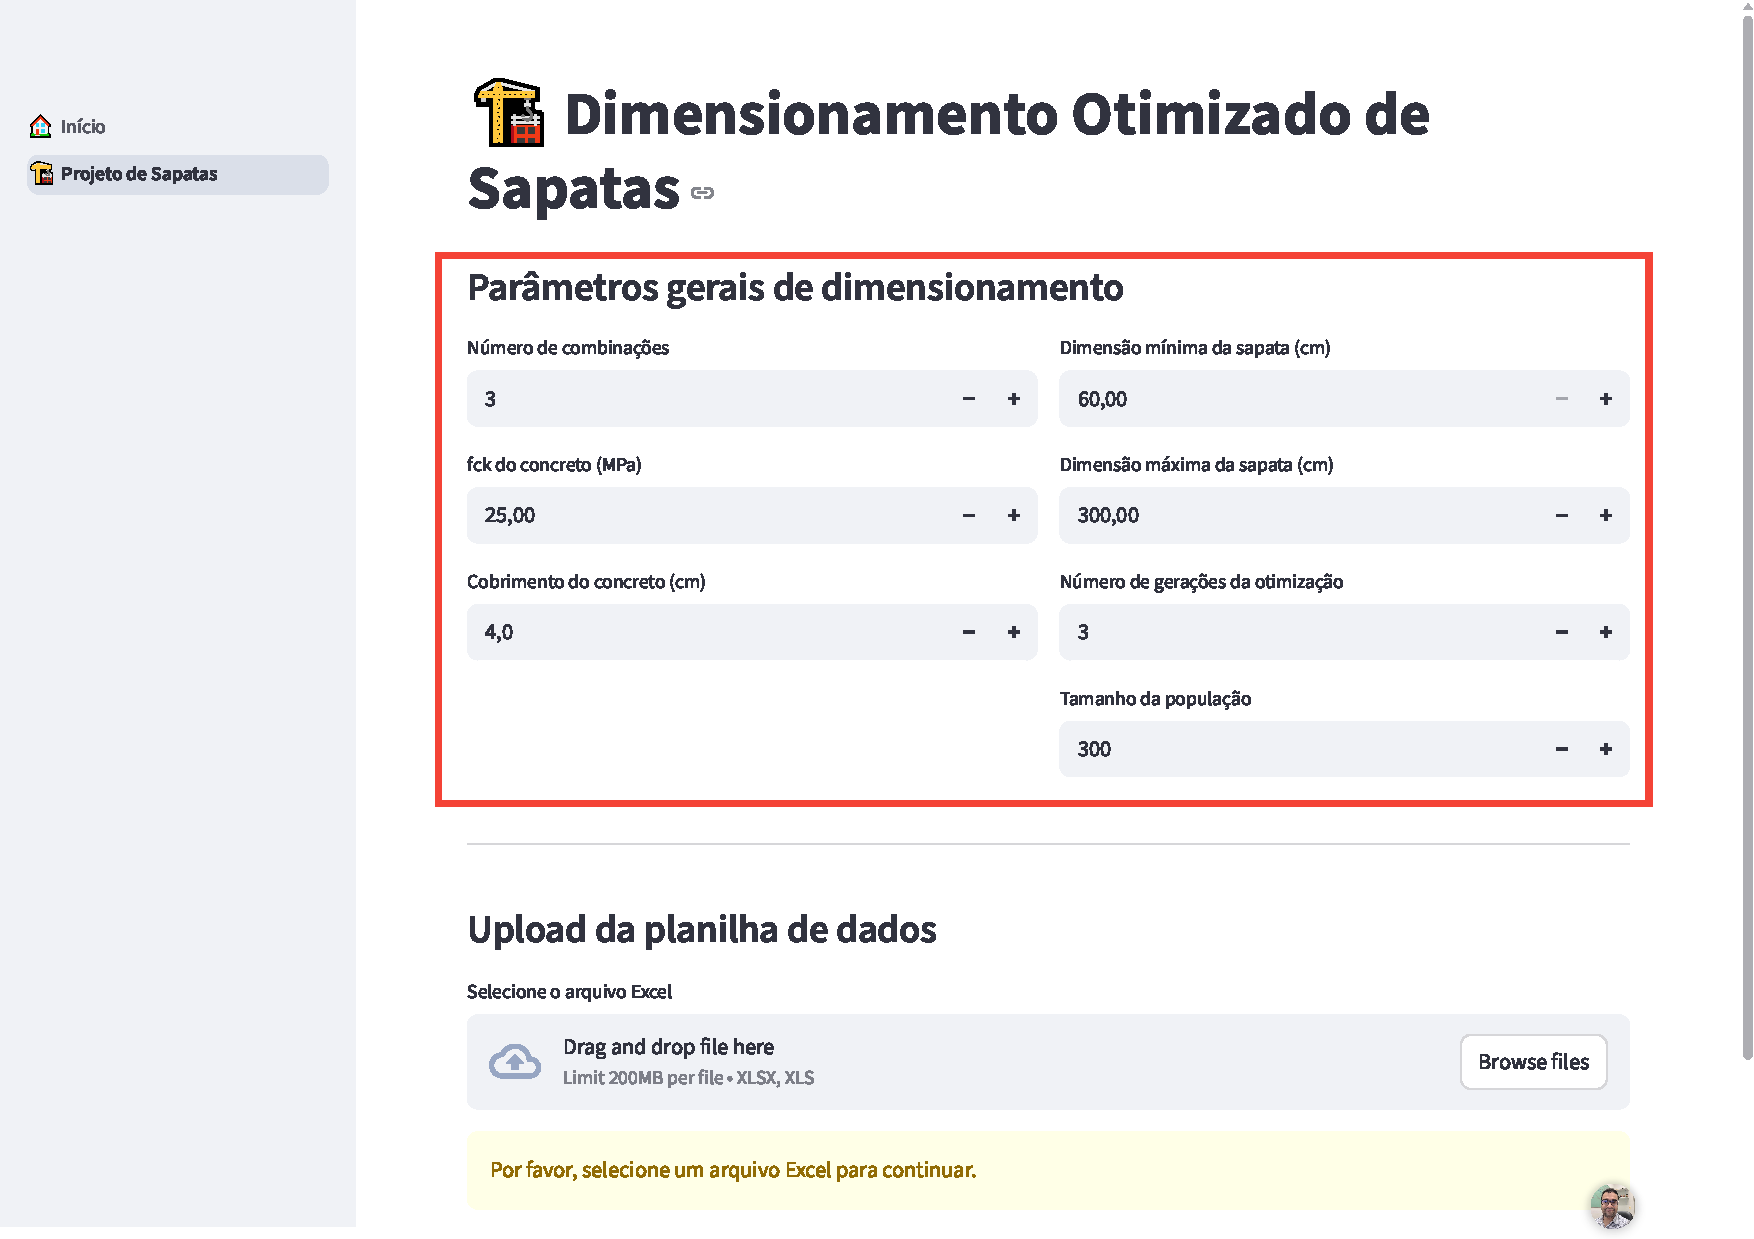
\includegraphics[width=1\linewidth]{figuras/pag_web_dados.pdf}
    \caption{Pagina de dimensionamento - Local da definição dos parâmetros.}
    \label{fig:pag_web_dados}
\end{figure}

\begin{figure}[htpb!]
    \centering
    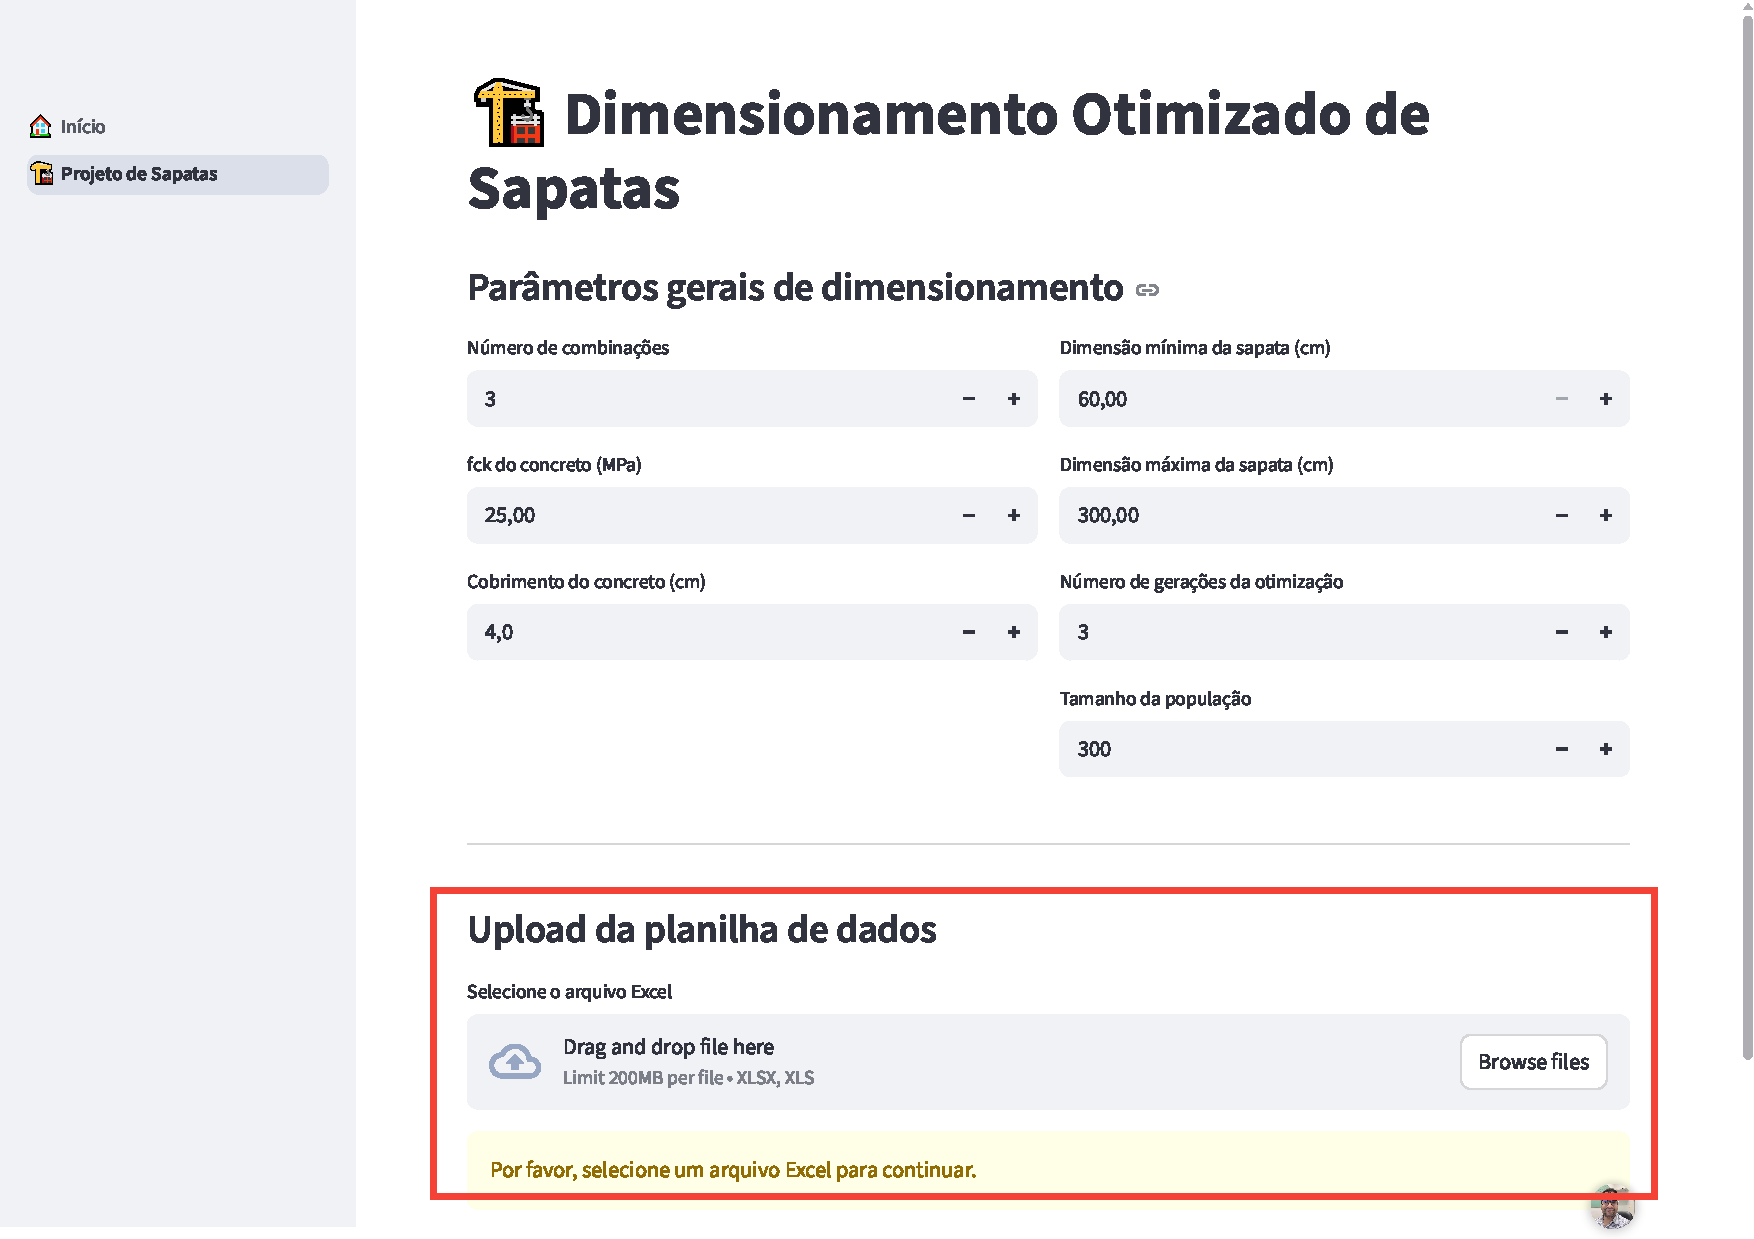
\includegraphics[width=1\linewidth]{figuras/pag_web_insercao.pdf}
    \caption{Pagina de dimensionamento - Local de inserção da planilha.}
    \label{fig:pag_web_insercao}
\end{figure}

Após a inserção dos dados de entrada, o usuário pode iniciar a execução do algoritmo por meio da interface gráfica, como aponta a Figura \ref{fig:pag_web_dimensionamento}. Durante o processamento, a ferramenta executa automaticamente as rotinas de cálculo conforme descritas ao longo deste trabalho. Ao final da execução, os resultados são apresentados ao usuário de forma organizada conforme mostra a Figura \ref{fig:pag_web_resultados} permitindo a visualização das dimensões ótimas obtidas para cada elemento de fundação e a possibilidade de baixar os resultados da rotina para os valores ótimos.

\begin{figure}[htpb!]
    \centering
    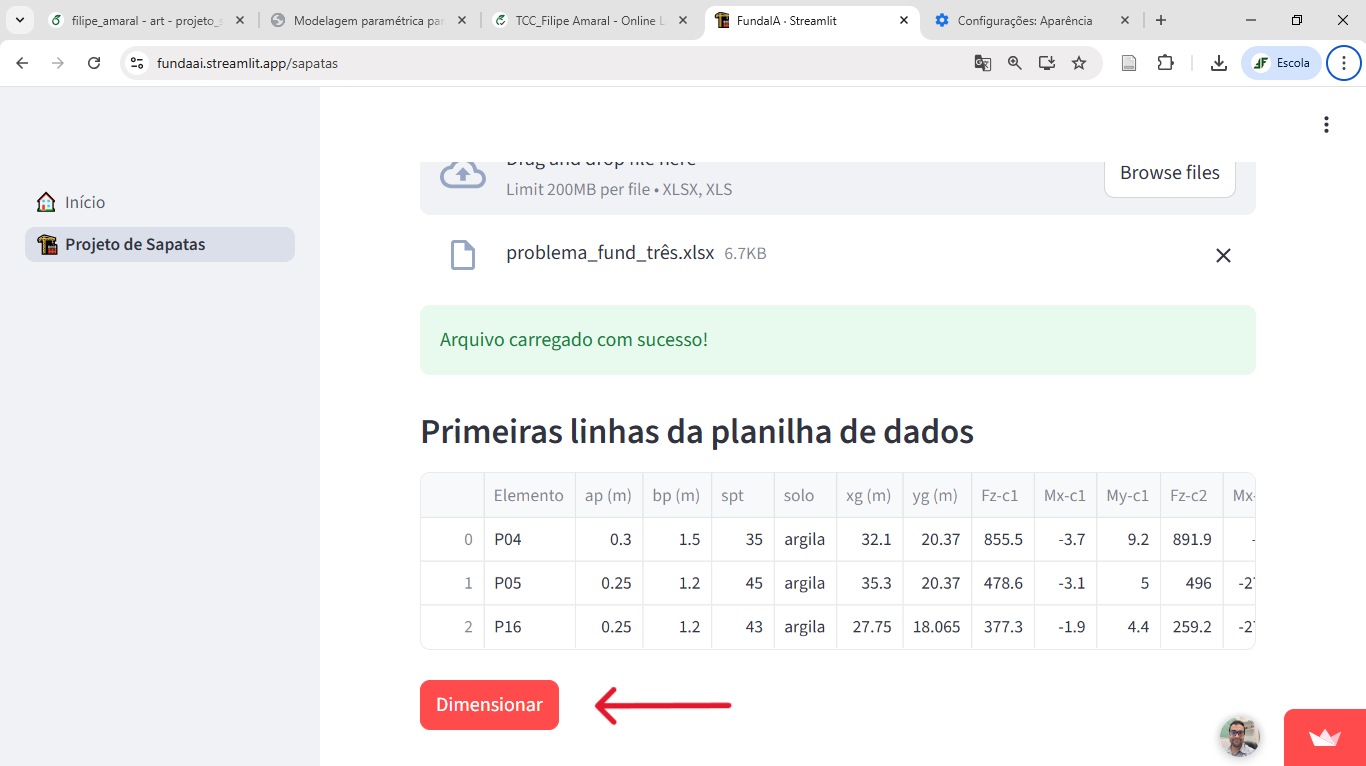
\includegraphics[width=1\linewidth]{figuras/pag_web_dimensionamento.png}
    \caption{Pagina de dimensionamento - Botão de dimensionamento.}
    \label{fig:pag_web_dimensionamento}
\end{figure}

\begin{figure}[htpb!]
    \centering
    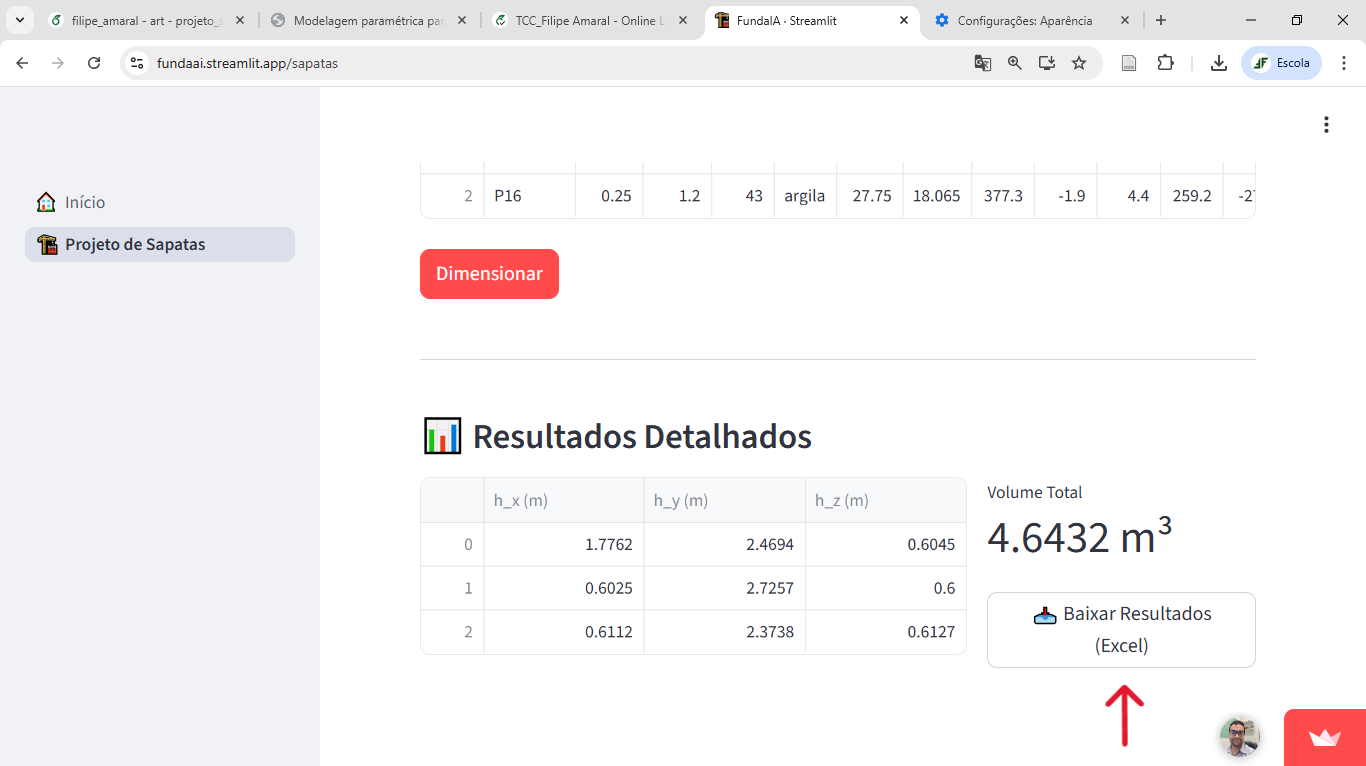
\includegraphics[width=1\linewidth]{figuras/pag_web_resultado.png}
    \caption{Pagina de dimensionamento - Resultados do dimensionamento.}
    \label{fig:pag_web_resultados}
\end{figure}


A ferramenta também disponibiliza a exportação dos resultados em formato de planilha, contendo as dimensões finais dos elementos dimensionados, juntamente com o conjunto detalhado das verificações realizadas para a solução ótima (ver Figura \ref{fig:pag_web_planilha}).  

% \begin{figure}[H]
%     \centering
%     \includegraphics[width=1\linewidth]{figuras/pag_web_planilha.png}
%     \caption{Planilha de resultados da otimização.}
%     \label{fig:pag_web_planilha}
% \end{figure}

\begin{figure}[htpb!]
    
    \centering
    \begin{subfigure}[b]{0.8\textwidth}
        \centering
        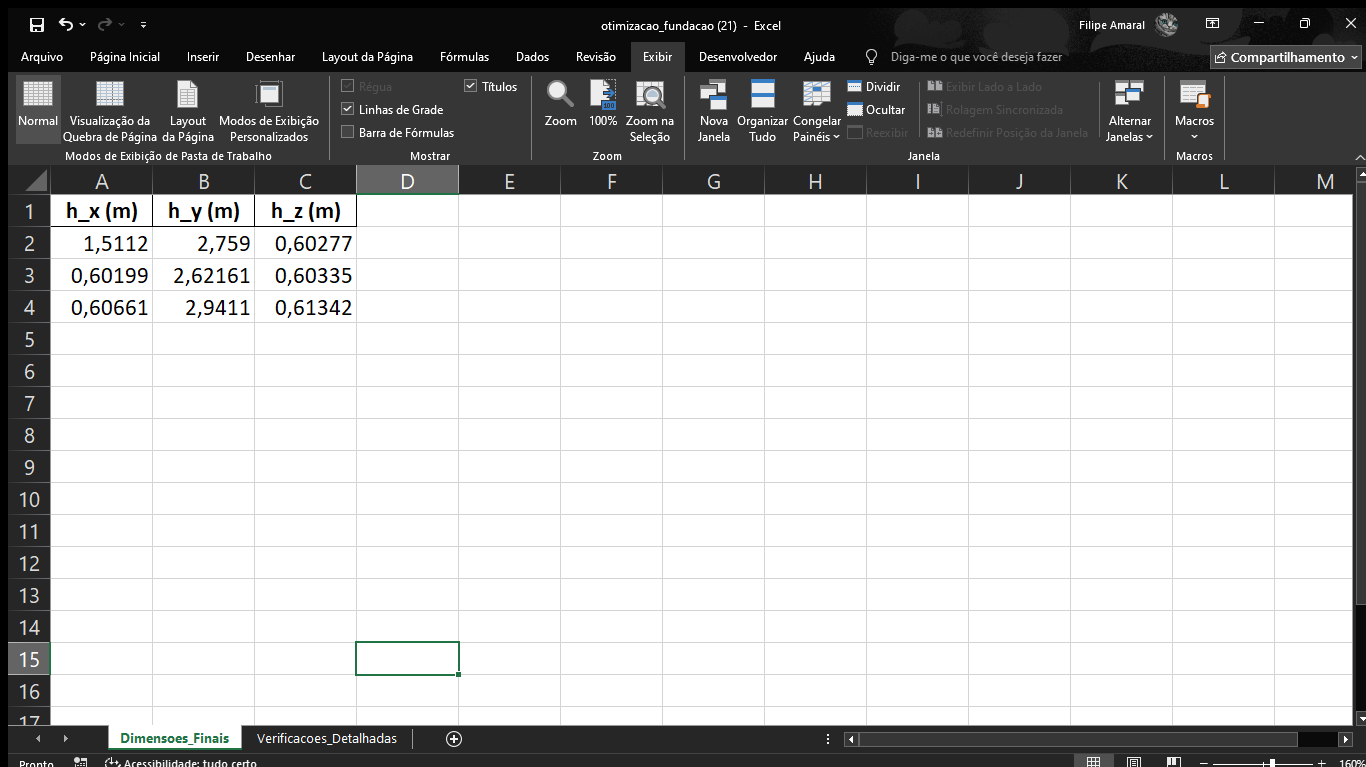
\includegraphics[width=\textwidth]{figuras/planilha a.png}
        \label{fig:exemplo_a}
    \end{subfigure}
    \hfill
    \begin{subfigure}[b]{0.8\textwidth}
        \centering
        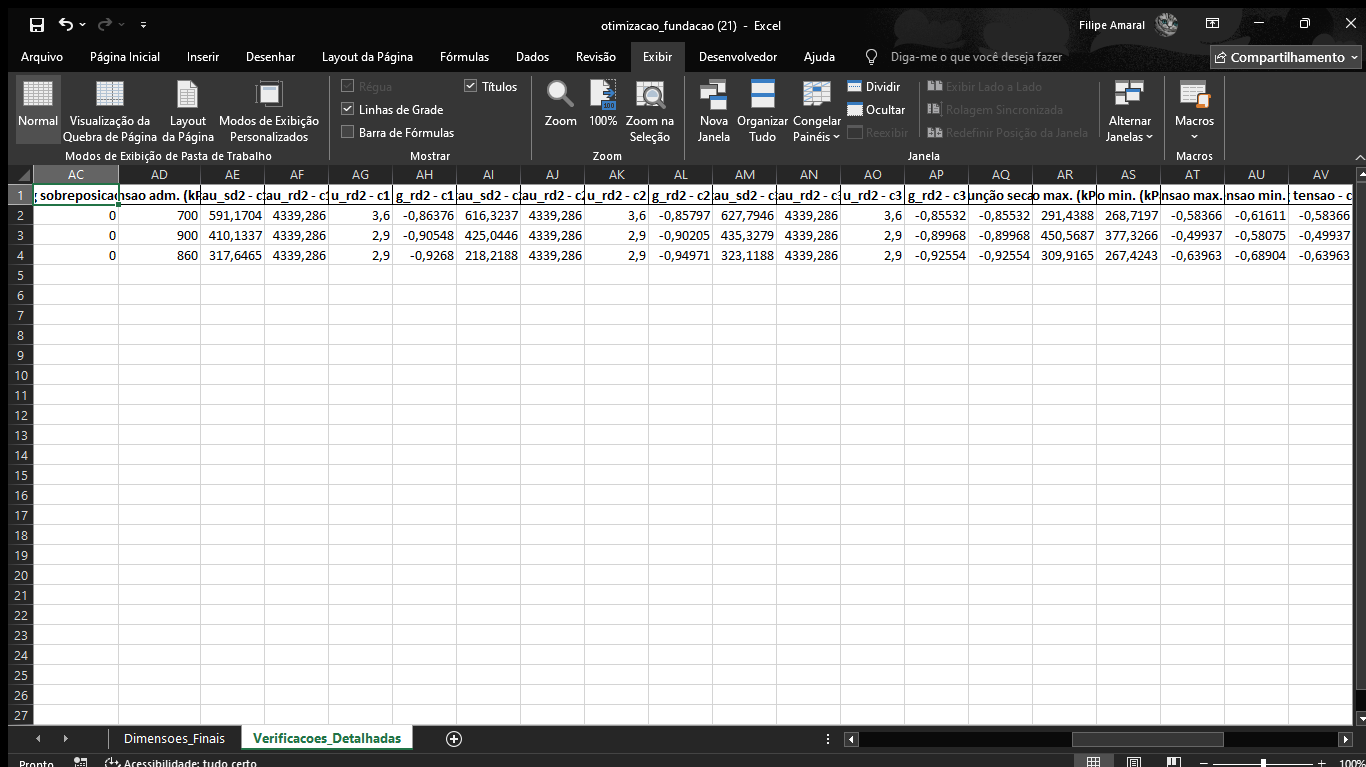
\includegraphics[width=\textwidth]{figuras/planilha b.png}

        \label{fig:exemplo_b}
    \end{subfigure}
    \caption{Planilha de resultados da otimização. (a) Dimensões ótimas e (b) Valores obtidos ao longo da verificação para as dimensões ótimas.}
    \label{fig:pag_web_planilha}
\end{figure}

\subsubsection{Resultado da otimização}

Nesta seção, são apresentados os resultados obtidos após a execução da ferramenta, ou seja, os resultados do dimensionamento otimizado. Para tanto, são empregados diferentes exemplos de projetos de fundações para demonstrar a real capacidade de uso do otimizador. Os exemplos são apresentados nas Seções seguintes, juntamente com seus respectivos resultados.

Para os processos de otimização, foi empregado o otimizador EGO (\textit{Efficient Global Optimization}), conforme descrito na Seção \ref{sec:ego}. Adotou-se uma população inicial de 300 elementos, com um número de gerações fixado em 3. O modelo substituto foi construído a partir de um processo gaussiano, no qual o \textit{kernel} foi definido de acordo com a estratégia apresentada na Seção~\ref{sec:desempenho_substituto}.

O problema de fundação consiste em um problema de 3 dimensões que correspondem as dimensões $h_x$, $h_y$ e $h_z$ da fundação. A função objetivo consiste na minimização do volume total das fundações analisadas, sendo a solução ótima definida pelo conjunto de dimensões que resulta no menor volume admissível, respeitando todas as restrições normativas e geométricas do problema. Todos esses exemplos foram executados pela interface disponível em\url{https://fundaai.streamlit.app/}.

% \paragraph{Fundação unica}
\subsubsubsection{Fundação única}

\label{item:um_elemento}

Para este exemplo utilizou-se apenas um único elemento para dimensionamento e otimização. As características do elemento estão expressas nas Tabelas \ref{tab:um_elemento} e \ref{tab:carga_um_elemento}.

\begin{table}[htbp!]
\centering
\caption{Características geométricas e do solo para o exemplo de uma fundação.}


\label{tab:um_elemento}
\setlength{\tabcolsep}{5pt}
\begin{tabular}{ c c c c c c c}
\toprule
\textbf{Elemento} &
$\mathbf{a_p \, (m)}$ &
$\mathbf{b_p \, (m)}$ &
$\mathbf{spt}$ &
$\mathbf{solo}$ &
$\mathbf{x_g \, (m)}$ &
$\mathbf{y_g \, (m)}$\\
\midrule
P08 & 2,10 & 0,25 & 12 & argila & 8,13 & 19,59 \\

\bottomrule
\end{tabular}
\end{table}

% Colocar aqui a tabela de cargas 
\begin{table}[htpb!]
\centering
\caption{Cargas atuantes para o exemplo de uma fundação.}
\label{tab:carga_um_elemento}
\setlength{\tabcolsep}{5pt}
\begin{tabular}{ c c c c c c c c c c}
\toprule
\textbf{Elemento} &
$\mathbf{F_{z,c1}}$ &
$\mathbf{M_{x,c1}}$ &
$\mathbf{M_{y,c1}}$ &
$\mathbf{F_{z,c2}}$ &
$\mathbf{M_{x,c2}}$ &
$\mathbf{M_{y,c2}}$ &
$\mathbf{F_{z,c3}}$ &
$\mathbf{M_{x,c3}}$ &
$\mathbf{M_{y,c3}}$ \\
\midrule
P08 & 857,40 & -0,20 & 115,60 & 913,00 & -0,90 & 0,10 & 950,60 & -0,90 & -0,50 \\

\bottomrule
\end{tabular}
\end{table}


Aplicando as informações na ferramenta, obtêm-se os valores otimizados: $h_x = 2,94\;m$, $h_y = 2,18\;m$, $h_z = 0,61\;m$ e $V = 3,91 \; m^3$. Os valores das restrições\footnote{ Os valores das restrições $g \le 0$ atendem aos critérios, enquanto $g > 0$ indicam desacordo. sendo que:

$g_{rd,2}^{ci}$: Restrição associada à verificação de punção na seção $C$ em função da combinação de carga $ci$; 

$g_{\sigma}^{ci}$: Restrição associada às tensões de contato entre a sapata e o solo para a combinação de carga $ci$; 

$g_{\mathrm{geom}}$: Restrição associada à compatibilidade geométrica entre o pilar e a sapata.} para o resultado encontrado, são apresentados na Tabela \ref{tab:resultado_g_uma_fundacao}.



% tabela de $g$ com a restrição mais impactante pintada de vermelho

\begin{table}[H]
\centering

\label{tab:resultado_g_uma_fundacao}
\begin{tabular}{cccccccccc}
\toprule
\textbf{Elemento} &
$\mathbf{g_{rd,2}^{c1}}$ &
$\mathbf{g_{rd,2}^{c2}}$ &
$\mathbf{g_{rd,2}^{c3}}$ &
$\mathbf{g_{\sigma}^{c1}}$ &
$\mathbf{g_{\sigma}^{c2}}$ &
$\mathbf{g_{\sigma}^{c3}}$ &
$\mathbf{g_{\mathrm{geom}}}$ \\
\midrule
 P08 & -0,90 & -0,89 & -0,89 & -0,01 & -0,19 & -0,15 & -0,07 \\
\bottomrule
\end{tabular}
\caption{Resultados das restrições para o problema de uma fundação.}
\end{table}

Considerando que a viabilidade é satisfeita ao alcançar $g \le 0$, observa-se na Tabela \ref{tab:resultado_g_uma_fundacao} que todas as restrições estruturais, geotécnicas e geométricas foram atendidas, não havendo nenhuma violação das condições impostas pelo problema. Para facilitar a interpretação dos resultados, aplicou-se a Equação \eqref{eq:solicitação/resistência}, que fornece a razão solicitação/resistência (S/R). Tal equação indica a razão de solicitação em função da resistência para as restrições que envolvem tensão, enquanto para as restrições que envolvem geometria, pode-se interpretar como valor necessário e valor permitido. Os resultados obtidos para todas as restrições são expressos na Tabela \ref{tab:S/R_uma_fundação}.


\begin{equation}
    \label{eq:solicitação/resistência}
    \frac{\text{Solicitação}}{\text{Resistência}} = \frac{Sd}{Rd} = g + 1
\end{equation}

\begin{table}[htpb!]
\centering
\caption{Razão Solicitação/Resistência (S/R) para as restrições para o problema de uma fundação.}
\label{tab:S/R_uma_fundação}
\begin{tabular}{cccccccccc}
\toprule
\textbf{Elemento} &
$\mathbf{g_{rd,2}^{c1}}$ &
$\mathbf{g_{rd,2}^{c2}}$ &
$\mathbf{g_{rd,2}^{c3}}$ &
$\mathbf{g_{\sigma}^{c1}}$ &
$\mathbf{g_{\sigma}^{c2}}$ &
$\mathbf{g_{\sigma}^{c3}}$ &
$\mathbf{g_{\mathrm{geom}}}$ \\
\midrule
P08 & 0,10	& 0,11	& 0,11	& 0,99	& 0,81	& 0,85	& 0,93 \\
\bottomrule
\end{tabular}
\end{table}

No que se refere as tensões de punção $g_{rd,2}^{c1}$, $g_{rd,2}^{c2}$ e $g_{rd,2}^{c3}$, os valores obtidos (-0,90; -0,89; -0,89) indicam elevada folga de resistência, como pode ser notado ao aplicar a Equação \eqref{eq:solicitação/resistência}, que resulta em valores na iguais a 0,10 a 0,11, ou seja, a solicitação de punção representa aproximadamente 11\% da resistência disponível. Esse comportamento evidencia que a punção não constitui a condição governante do dimensionamento, apresentando uma margem de segurança significativamente superior à necessária para a viabilidade estrutural. Além disso, os valores para cada combinação apresentaram leve variação, indicando que a variação de $F_{zk}$ surte pouca influência para essa restrição. 

Por outro lado, as restrições associadas às tensões no solo obtiveram um comportamento distinto. A combinação $g_{\sigma}^{c1}$ = -0,01 corresponde a uma razão S/R de 0,99, o que caracteriza que tal restrição teve maior impacto no processo de otimização (uma solicitação de 99\% da tensão admissível). As combinações $c2$ e $c3$, com valores de razão solicitação/resistência de 0,81 e 0,85, apresentam folgas moderadas, mas substancialmente inferiores as apreciadas na verificação à punção.

A restrição geométrica $g_{\mathrm{geom}} = -0,07$ também se encontra satisfeita, indicando o atendimento às exigências, com relativa folga, uma vez que, pela Equação \eqref{eq:solicitação/resistência}, obtém-se uma razão de 0,93, que, embora represente um valor alto, não ultrapassa a restrição de tensão. 

A analise percentual das razões S/R entre a restrição mais dominante e a menos solicitada (Equação \eqref{eq:analise_gsc1_gp_c1}) evidencia que a restrição de tensão $g_{\sigma}^{c1}$ apresenta solicitação 890\% superior à verificada para a restrição de punção $g_{rd,2}^{c1}$, a qual corresponde a mais negativa. 



\begin{equation}
    \label{eq:analise_gsc1_gp_c1}
    \frac{0,99-0,10}{0,10} \cdot 100 = 890\%
\end{equation}

Assim, conclui-se que a restrição de tensão solo-sapata $g_{\sigma}^{c1}$ é a condição governante para o processo de dimensionamento e otimização, sendo responsável por limitar o espaço de busca para as dimensões em planta.

Quando comparada às demais combinações de tensão no solo (Equações \eqref{eq:analise_gsc1_gsc2} e \eqref{eq:analise_gsc1_gsc3}), verifica-se que a combinação $c1$ impõe uma solicitação entre 16,57\% e 22,22\% superior às combinações $c2$ e $c3$, respectivamente. Esses resultados demonstram, de forma inequívoca, que a condição $g_{\sigma}^{c1}$ constitui a restrição governante do problema de otimização para essa configuração.

\begin{equation}
    \label{eq:analise_gsc1_gsc2}
    \frac{0,99-0,81}{0,81} \cdot 100 = 22,22 \%
\end{equation}

\begin{equation}
    \label{eq:analise_gsc1_gsc3}
    \frac{0,99-0,85}{0,85} \cdot 100 = 16,47\%
\end{equation}


% Executando-se o dimensionamento para  o mesmo elemento, considerando as condições de escritório, ou seja, através de tentativa e erro (foi usada uma amostragem de Monte Carlo para essa simulação, como explicitado no Item \ref{subsubsub:comparacao}), obteve-se um resultado com o volume final de 7,71 $m^3$. Para tanto, foram preparadas 200 tentativas, o que, em um escritório de engenharia, exigiria elevado esforço por parte dos profissionais e um alto grau de organização das planilhas de cálculo. E, contudo, obtiveram-se resultados menos econômicos, uma vez que o valor final foi maior que o obtido pela otimização, de 3,91 m³.

\subsubsubsection{Três elementos de fundação}
\label{item:tres_elemento}

Para este exemplo, utilizou-se um conjunto de três elementos com o intuito de dimensioná-los e otimizá-los. Tal conjunto corresponde aos elementos do problema tratado na Seção \ref{sec:problema_brinquedo} deste trabalho e, assim, suas características estão expressas nas Tabelas \ref{tab:valores_geometricos_reais} e \ref{tab:carga_atuante_real}.


Aplicando as informações na ferramenta \textit{web}, obtém-se os valores otimizados apresentados na Tabela \ref{tab:dimensoes_3_fundacoes}. Foram obtidos os valores das restrições para os resultados encontrados são apresentados na Tabela~\ref{tab:resultado_g_3_fundacoes}.

% tabela de resultado hx hy e hz

\begin{table}[H]
\centering
\caption{Dimensões finais para o problema de 3 fundações.}
\label{tab:dimensoes_3_fundacoes}
\begin{tabular}{ccccc}
\toprule
\textbf{Elemento} &
$\mathbf{h_x\,(m)}$ &
$\mathbf{h_y\,(m)}$ &
$\mathbf{h_z\,(m)}$ &
$\mathbf{V\,(m^3)}$\\
\midrule
P04 & 1,73 & 2,37 & 0,60 & 4,70\\
P05 & 0,62 & 2,72 & 0,60 & 1,01\\
P16 & 2,61 & 1,42 & 0,63 & 2,33\\
\bottomrule
\end{tabular}
\end{table}

% tabela de g com restrição mais impactante pintada de vermelho

\begin{table}[H]
\centering
\caption{Resultados das restrições para o problema de 3 fundações.}
\label{tab:resultado_g_3_fundacoes}
\begin{tabular}{ccccccccc}
\toprule
\textbf{Elemento} &
$\mathbf{g_{rd,2}^{c1}}$ &
$\mathbf{g_{rd,2}^{c2}}$ &
$\mathbf{g_{rd,2}^{c3}}$ &
$\mathbf{g_{\sigma}^{c1}}$ &
$\mathbf{g_{\sigma}^{c2}}$ &
$\mathbf{g_{\sigma}^{c3}}$ &
$\mathbf{g_{\mathrm{geom}}}$ \\
\midrule
P04 & -0,86 & -0,86 & -0,86 & -0,58 & -0,48 & -0,51 &  -0,45 \\
P05 & -0,91 & -0,90 & -0,90 & -0,54 & -0,32 & -0,31 &  -0,70 \\
P16  & -0,93 & -0,95 & -0,93 & -0,83 & -0,86 & -0,81 &  -0,01 \\
\bottomrule
\end{tabular}
\end{table}

Aplicou-se a Equação \eqref{eq:solicitação/resistência} aos valores correspondentes às restrições avaliadas, a fim de construir a Tabela \ref{tab:S/R_tres_fundação}, na qual é apresentada a razão S/R para cada verificação.

\begin{table}[htpb!]
\centering
\caption{Razão Solicitação/Resistência (S/R) para as restrições do problema de três fundações.}
\label{tab:S/R_tres_fundação}
\begin{tabular}{cccccccccc}
\toprule
\textbf{Elemento} &
$\mathbf{g_{rd,2}^{c1}}$ &
$\mathbf{g_{rd,2}^{c2}}$ &
$\mathbf{g_{rd,2}^{c3}}$ &
$\mathbf{g_{\sigma}^{c1}}$ &
$\mathbf{g_{\sigma}^{c2}}$ &
$\mathbf{g_{\sigma}^{c3}}$ &
$\mathbf{g_{\mathrm{geom}}}$ \\
\midrule
P04 & 0,14 & 0,14 & 0,14 & 0,42 & 0,52 & 0,49 & 0,55 \\
P05 & 0,09 & 0,10 & 0,10 & 0,46 & 0,68 & 0,69 & 0,30 \\
P16 & 0,07 & 0,07 & 0,05 & 0,07 & 0,17 & 0,14 & 0,99 \\
\bottomrule
\end{tabular}
\end{table}

A analise das verificações à punção ($g_{rd,2}^{c1}$, $g_{rd,2}^{c2}$ e $g_{rd,2}^{c3}$) evidencia que a razão S/R apresenta elevada folga de resistência para todas as restrições, com valores compreendidos entre 0,05 e 0,14, ou seja, correspondendo à uma solicitação de no máximo 14\% da resistência à punção. Tal resultado indica que a punção não constitui uma condição governante do dimensionamento para esta configuração. Ademais, observa-se pequena variação das restrições entre as combinações de carregamento para um mesmo elemento, reafirmando que a variação de $F_{zk}$ exerce pouca influência sobre essa restrição ou que a dimensão $h_z$ foi suficientemente grande para amortecer os efeitos de tal variação. 

Quanto às tensões de contato com o solo, os valores para as verificações situam-se com razão S/R entre 0,07 e 0,69, correspondendo a solicitações de no máximo 69\% da capacidade de suporte do solo. Observa-se que o elemento P16 tem valores mais baixos, na faixa de 0,07 a 0,17, enquanto os elementos P04 e P05 encontram-se entre 0,42 e 0,69, indicando que, para estes últimos, o efeito geotécnico foi aproximadamente 306\% mais determinante do que para o elemento P16, conforme expresso na Equação \eqref{eq:analise_gsc3_gsc2}. Esse resultado evidencia que, para o elemento P05, com 69\% de solicitação, tem-se a restrição $g_{\sigma}^{c3}$ como a mais solicitante entre as restrições geotécnicas.

\begin{equation}
    \label{eq:analise_gsc3_gsc2}
    \frac{0,69-0,17}{0,17}\cdot100= 305,88\%
\end{equation}

Porém, diferente do problema de uma única fundação, no qual o critério geotécnico era governante no dimensionamento, observa-se que, neste arranjo com três fundações, a limitação geométrica assume um papel determinante no processo de otimização. A restrição $g_{geom}$ apresenta razões S/R iguais a 0,55, 0,30 e 0,99. Nota-se que o elemento P16 encontra-se no limite geométrico, configurando-se como a restrição governante para o arranjo.

A comparação entre a maior razão observada (0,99) e a menor razão global registrada (0,05) resulta em diferença percentual de aproximadamente 1880\%, conforme indicado na Equação \eqref{eq:analise_ggeom_gp16c3}. Tal discrepância reforça a predominância da condição geométrica no controle da solução ótima, evidenciando que o processo de minimização volumétrica conduz o elemento P16 ao limite geométrico antes que as demais verificações se tornem críticas.

\begin{equation}
    \label{eq:analise_ggeom_gp16c3}
    \frac{0,99-0,05}{0,05}\cdot100= 1880\%
\end{equation}

A análise das razões permite observar que apenas um dos três elementos teve restrição que alcançou valor próximo do limite (99\% para a restrição geométrica de P16), caracterizando-se como restrição governante. Os demais elementos (P04 e P05) apresentam margens significativas em suas verificações. Esse comportamento  demonstra que a formulação adotada conduz a uma solução ótima global, na qual nem todos os elementos atingem o limite individual. Assim, embora P04 e P05 apresentem potencial para a redução de dimensões quando analisados individualmente, tal redução pode não ser significativa para o benefício global. 

Por fim, neste arranjo com três elementos, a configuração espacial, com leve grau de proximidade, permitiu que o otimizador evitasse a existência de sobreposição, contrastando com o problema da Seção \ref{sec:problema_brinquedo} em que foi apresentada sobreposição.

\subsubsubsection{Consideração para um regime com elementos sobrepostos}
\label{item:elemento_sobreoposto}

Nesta seção é apresentada a otimização de elementos com alto grau de proximidade, com o objetivo de analisar e demonstrar o comportamento da ferramenta nessas situações específicas. As Tabelas \ref{tab:dois_elemento} e \ref{tab:carga_2_elementos} apresentam os dados iniciais para o dimensionamento.

\begin{table}[H]
\centering
\caption{Características geométricas e do solo para o exemplo de duas fundações.}
\label{tab:dois_elemento}
\setlength{\tabcolsep}{5pt}
\begin{tabular}{ c c c c c c c}
\toprule
\textbf{Elemento} &
$\mathbf{a_p \, (m)}$ &
$\mathbf{b_p \, (m)}$ &
$\mathbf{spt}$ &
$\mathbf{solo}$ &
$\mathbf{x_g \, (m)}$ &
$\mathbf{y_g \, (m)}$\\
\midrule
P01 & 0,25 & 1,20 & 10 & argila & 6,90 & 26,255 \\
P02 & 0,30 & 1,50 & 12 & argila & 7,985 & 25,105 \\
\bottomrule
\end{tabular}
\end{table}

\begin{table}[H]
\centering
\caption{Carregamentos atuantes por combinação}
\label{tab:carga_2_elementos}
\begin{tabular}{cccccccccc}
\toprule
\textbf{Elemento} &
$\mathbf{F_{z}^{c1}}$ &
$\mathbf{M_{x}^{c1}}$ &
$\mathbf{M_{y}^{c1}}$ &
$\mathbf{F_{z}^{c2}}$ &
$\mathbf{M_{x}^{c2}}$ &
$\mathbf{M_{y}^{c2}}$ &
$\mathbf{F_{z}^{c3}}$ &
$\mathbf{M_{x}^{c3}}$ &
$\mathbf{M_{y}^{c3}}$ \\
\midrule
P01 & 485,9 & -0,3 & 4,1 & 511,6 & -32,4 & -0,4 & 511,6 & -32,4 & -0,4 \\
P02 & 885,8 & -1,0 & 9,2 & 912,1 & -65,4 & 0,1  & 915,9 & -40,0 & 0,1  \\
\bottomrule
\end{tabular}
\end{table}


Aplicando as informações na ferramenta, foram obtidos os resultados expressos nas Tabelas \ref{tab:dimensoes_2_fundacoes} e \ref{tab:resultado_g_2_fundacoes}.

\begin{table}[H]
\centering
\caption{Dimensões finais para o problema de 2 fundações.}
\label{tab:dimensoes_2_fundacoes}
\begin{tabular}{ccccc}
\toprule
\textbf{Elemento} &
$\mathbf{h_x\,(m)}$ &
$\mathbf{h_y\,(m)}$ &
$\mathbf{h_z\,(m)}$ &
$\mathbf{V\,(m^3)}$\\
\midrule
P01 & 2,99 & 1,40 & 0,61 & 2,55\\
P02 & 3,00 & 1,90 & 0,61 &  3.48\\
\bottomrule
\end{tabular}
\end{table}




\begin{table}[H]
\centering
\caption{Resultados das restrições para o problema de 2 fundações.}
\label{tab:resultado_g_2_fundacoes}
\begin{tabular}{ccccccccccc}
\toprule
\textbf{Elemento} &
$\mathbf{g_{\textbf{sobreposição}}}$ &
$\mathbf{g_{rd,2}^{c1}}$ &
$\mathbf{g_{rd,2}^{c2}}$ &
$\mathbf{g_{rd,2}^{c3}}$ &
$\mathbf{g_{\sigma}^{c1}}$ &
$\mathbf{g_{\sigma}^{c2}}$ &
$\mathbf{g_{\sigma}^{c3}}$ &
$\mathbf{g_{\sigma}}$ &
$\mathbf{g_{\mathrm{geom}}}$ \\
\midrule
P01 & 0,23 &-0,90 &	-0,90	& -0,90 & -0,18 & -0,06 & -0,06 & -0,06 & 0,00 \\
P02 & 0,18 & -0,86 & -0,86 & -0,86 & -0,08 & 0,04 & 0,00 & 0,04 & -0,1 \\
\bottomrule
\end{tabular}
\end{table}

A análise da Tabela \ref{tab:resultado_g_2_fundacoes} evidencia que a configuração do problema com duas fundações apresentam violação da restrição de sobreposição, com valores de $g_{\text{sobreposição}}$ iguais a 0,23 e 0,18 para os elementos P01 e P02, respectivamente. Como valores positivos indicam a extrapolação do domínio viável, conclui-se que ambas as fundações não satisfazem a questão de sobreposição, indicando que as dimensões em planta interferem entre si no arranjo espacial.

Ao analisar a Tabela \ref{tab:S/R_duas_fundação}, obtida a partir da aplicação da Equação \eqref{eq:solicitação/resistência}, percebe-se que as verificações à punção estão na faixa de 10 a 14\% de solicitação da resistência estrutural, confirmando que essa restrição não exerce influência determinante no dimensionamento para esta configuração.


\begin{table}[htpb!]
\centering
\caption{Razão Solicitação/Resistência (S/R) para as restrições do problema de duas fundações.}
\label{tab:S/R_duas_fundação}
\begin{tabular}{ccccccccccc}
\toprule
\textbf{Elemento} &
$\mathbf{g_{\textbf{sobreposição}}}$ &
$\mathbf{g_{rd,2}^{c1}}$ &
$\mathbf{g_{rd,2}^{c2}}$ &
$\mathbf{g_{rd,2}^{c3}}$ &
$\mathbf{g_{\sigma}^{c1}}$ &
$\mathbf{g_{\sigma}^{c2}}$ &
$\mathbf{g_{\sigma}^{c3}}$ &
$\mathbf{g_{\mathrm{geom}}}$ \\
\midrule
P01 & 1,30 & 0,10 & 0,10 & 0,10 & 0,82 & 0,94 & 0,94 & 1,00 \\
P02 & 1,18 & 0,14 & 0,14 & 0,14 & 0,92 & 1,04 & 1,00 & 0,90\\
\bottomrule
\end{tabular}
\end{table}

Quanto às tensões de contato entre a sapata e o solo, observa-se que o elemento P02 apresenta um valor positivo para a combinação $c2$, com $g_{\sigma}^{c2}$ igual a 0,04, o que corresponde uma uma razão S/R de 1,04, assim caracterizando uma violação da tensão admissível, com uma solicitação de 104\% da tensão resistente. As demais verificações de tensão permanecem no domínio viável, com razões S/R entre 0,82 e 1,00, indicando que algumas combinações encontram-se próximas do limite, bem como no limiar da viabilidade, embora não tenham ultrapassado.

Além disso, observa-se que a verificação de geometria apresenta valores de razão S/R na ordem de 0,90 e 1,00, evidenciando que os elementos estão próximos do limite dimensional permitido. Tal comportamento indica que o processo de otimização conduziu as dimensões em planta a valores limítrofes.

Constata-se que, devido ao alto grau de sobreposição entre os elementos, o otimizador reduziu progressivamente as dimensões, aproximando-as do limite geométrico admissível.  Entretanto, essa redução implicou no aumento das tensões de contato no solo, culminando na violação observada para o elemento P02. Ainda assim, mesmo com a diminuição das dimensões, a solução obtida não foi suficiente para eliminar completamente a sobreposição, evidenciando um conflito entre as restrições espaciais e geotécnicas na configuração analisada.

Por fim, observa-se que a ferramenta é capaz de identificar a ocorrência de sobreposição entre os elementos de fundação e de buscar alternativas para mitigar essa condição ao longo do processo de otimização. Contudo, devido ao alto grau de sobreposição, a estratégia de alterar as dimensões da sapata não foi suficiente para contornar os efeitos severos da sobreposição. Porém, ao explorar resultados que convergem nas outras restrições, a ferramenta possui potencial para questões de pré dimensionamento.


\subsubsection{Comparação de resultados obtidos por força bruta}
\label{subsubsub:comparacao}

Realizou-se o dimensionamento dos mesmos elementos aplicados nas Seções \ref{item:um_elemento}, \ref{item:tres_elemento} e \ref{item:elemento_sobreoposto}, seguindo o método de Monte Carlo (MMC), com o objetivo de reproduzir resultados equivalentes àqueles usualmente obtidos na prática de escritório. Tal prática caracteriza-se pela adoção de procedimentos iterativos baseados em tentativa e erro, nos quais sucessivas combinações de parâmetros são avaliadas até que se obtenham soluções admissíveis segundo os critérios de projeto.

Para alcançar soluções admissíveis pelo MMC foram necessárias 200 tentativas. Em um contexto profissional não necessita-se de tal volume de iterações. Contudo, ainda demandaria elevado esforço técnico, um significativo dispêndio de tempo e um alto grau de organização das planilhas de cálculo. Mesmo diante desse volume de trabalho, o resultado obtido mostrou-se pouco econômico quando comparado aos resultados produzidos pela metodologia de otimização. Ademais, no ambiente de escritório, o tempo disponível e a carga de trabalho do profissional podem influenciar diretamente o resultado final, uma vez que o projetista pode se dar por satisfeito antes de atingir a solução mais eficiente possível. Neste sentido, a Tabela \ref{tab:volume_final} traz a comparação dos resultados obtidos pelo método Monte Carlo e pela metodologia proposta, através da aplicação  da Equação \eqref{eq:diferenca_percentual}.

\begin{equation}
    \label{eq:diferenca_percentual}
    \text{Redução percentual}\;(\%) = \frac{V_{MMC} - V_{otimizado}}{V_{MMC}} \cdot 100
\end{equation}

\begin{table}[H]
\centering
\caption{Redução dos volumes obtidos pelo metodologia proposta em relação com o método tradicional.}
\label{tab:volume_final}
\begin{tabular}{ccccc}
\toprule
\textbf{Elemento} &
$\mathbf{V_{MMC}\;(m^3)}$ &
$\mathbf{V_{otimizado}\;(m^3)}$ &
\textbf{Volume reduzido} $(\%)$ \\
\midrule
P01 & 5,34 & 2,55 & 52,25 \\
P02 & 4,04 & 3,48 & 13,86 \\
P04 & 3,82 & 4,70 &  -23,04\\
P05 &  7,15 & 1,01 &  85,87\\
P08 & 7,72 & 3,91 &  49,35 \\
P16 & 6,94 & 2,33 & 66,43 \\
\bottomrule
\end{tabular}
\end{table}

A metodologia proposta demonstra uma clara vantagem ao explorar, de forma sistemática, o espaço de soluções, reduzindo a dependência de decisões subjetivas e conduzindo a resultados significativamente mais econômicos e consistentes na maioria dos elementos, alcançando uma redução média de 40,79\%. Contudo, o elemento P04 apresentou desempenho inferior em termos de redução de volume.